\documentclass[twoside]{uocthesis}

\usepackage{graphicx}
\frenchspacing

\Title{Repeatability of Pre-Flashover Fire Patterns on Gypsum Wall Board}
\Author{Daniel Madrzykowski}
\Year{2015}

\Supervisor{Dr Charles Fleischmann}
\Department{Department of Fire Safety Engineering}

\begin{document}

\bibliographystyle{unsrt}

\prelimpages

\titlepage

\dedication{To my wife and family}

\abstract{
Uncontrolled fires result in loss of life, property and can create an adverse economic impact on a community.  The investigation of fires provides a means to identify the cause of the fire in order to develop a knowledge base that could enable the elimination of that cause and thus reduce the losses from fires.  However, as the result of the review of several arson cases and a review by the U.S. National Academy of Sciences, questions about the lack of the use of science in the practice of fire investigation were raised.  Specifically the National Academy of Sciences indicated that ``... research is needed on the natural variability of burn patterns...''
This study addresses that need in two ways:
\begin{enumerate}
\item Examining the repeatability of several small fire sources and the fire patterns that were generated by those fires
\item Examining the capability of using numerical models to simulate the fires and the resulting fire patterns based on input data collected from engineering reference sources, and bench scale and full scale fire experiments conducted in this study.
\end{enumerate}
This paper highlights the many uncertainties involved in what appear to be simple fire experiments.  A variety of uncertainties related to the composition of the fuels, measurement methods, and analysis techniques just to list a few of the areas considered.  The objective of the research was to examine the repeatability of pre-flashover fire patterns generated from exposure to short duration (300 s maximum) well characterized fires.  Three different fuels were used: natural gas, gasoline, and polyurethane foam.  Each fuel had a similar top surface area.  The heat release rate data showed that the variability was greater for more complex fuels.  While the variation in peak heat release rate with the natural gas was similar to the expanded uncertainty of the measurement system, 11~\%, the variation in the peak heat release rates of the gasoline and the polyurethane foam increased due to increased uncertainties in the burning behavior of the fuels.  The patterns generated by the polyurethane foam fire, had more variability than the natural gas and the gasoline fire patterns.  This is likely due to the greater variability of the burning of the solid fuel and the lower heat release rate.  The maximum fire pattern heights generated from the natural gas and gasoline fires were shown to have uncertainties of 18~\% or less based on a Type A statistical analysis with 95~\% confidence limits.  The comparison of the fire pattern heights and the mean flame height demonstrated that the ``'steady state'' natural gas fires exhibited the highest level of agreement and polyurethane foam fueled fire exhibited the least agreement, with the gasoline fueled fires in between.

This trend is the same as exhibited by the repeatability of the heat release rate measurements and the flame height measurements.   *****Computational results here ****

}

\tableofcontents

\listoffigures

\listoftables

\acknowledgments{
I would like to thank Prof.~Fleishmann, etc.

This work was partially funded by the National Institute of Justice (NIJ) through an interagency agreement with the NIST Office of Law Enforcement Standards (OLES). I would like to thank Susan Ballou of OLES for her support of this project. This work was also partially supported by the U.S. Fire Administration.

The would also like to thank Roger Nokes for his development and continued assistance with Streams and to the New Zealand Fire Commission for their financial support to the University of Canterbury

Finally, my family...
}

\textpages

\chapter{Introduction}
\label{chapter:Introduction}

Uncontrolled fires result in loss of life, property and can create an adverse economic impact on a community.  Findings from an archaeological site in South Africa, published in 2012, indicate that mankind has productively used fire for approximately 1 million years~\cite{Berna:2012}.  This is 300 thousand years earlier than previously thought.  Despite mankind’s extensive history with fire, according to the World Health Organization, an estimated 265,000 people die each year as a result of burn injuries~\cite{WHO:2014}.  Based on an estimated global population of 7.3 billion people, the death rate due to burns from all sources would be 3.6 per 100,000 populations.  The World Fire Statistics Center collects data from European, North American and a few Asia-Oceania countries.  Within this group of countries the fire deaths per 100,000 population range from 0.02 (Singapore) to 2.03 (Finland)~\cite{Climate:2014}. There are a significant number of factors that determine the variability of fire death rates between nations, socio-economic conditions being a leading factor~\cite{WHO:2014}.

In the United States, the loss of life due to unwanted fire has been decreasing steadily since the 1970’s.  This is neglecting the increased loss of life as a result of the terrorist attack on September 11, 2001.  The estimated number of fire deaths in the U.S. in 1975 was 8,100 or 3.75 deaths per 100,000 population~\cite{America_Burning_Revisited}.  In 2013, there were 3,240 civilian fire fatalities or 1.02 deaths per 100,000 population~\cite{Karter:2014}.  During this same period, the number of fires in the United States has decreased from 2.5 million fires to 1.24 million fires.  There are many reasons that led to this decrease in loss of life due to fire in the United States.  An example would be research and data that enabled the development of product safety standards, improved building codes, improved fire safety systems, and fire prevention programs to name just a few.  None of this happened without the constant effort of agencies at the Federal, state, and, local levels working with professional fire organizations to deliver the five E’s of fire prevention; Engineering, Education, Enforcement, Economic Incentive, and Emergency Response~\cite{FIVE}.

Fire investigation is a key element in the fire prevention system that generates data to enable the reduction of fire losses.  The investigation of fires provides a means to identify the cause of the fire in order to develop a knowledge base that could enable the elimination of that cause and thus further reduce the losses from fires.  Data such as the room of fire origin, the first item ignited and ultimately the cause of the fire is information that is critical to understanding and reducing the number of fires.  For example, the identification of products that are involved in ignitions due to a design flaw, in many cases result in the U.S. Consumer Product Safety Commission or a manufacturer issuing a product recall.
In some cases, the fire investigation determines that the fire was intentional.  An intentional fire as defined in the National Fire Incident Reporting System (NFIRS)  are those fires that are deliberately set and include fires that result from deliberate misuse of a heat source, fires of an incendiary nature (arson), as well as controlled burn fires, such as crop clearing, that required fire service intervention~\cite{Campbell:2014}.  An incendiary fire, as defined by the National Fire Protection Association (NFPA) Guide for Fire \& Explosion Investigations, commonly referred to as NFPA~921, is ``a fire that is deliberately set with the intent to cause a fire to occur in an area where the fire should not be.''~\cite{NFPA_921}.

According to the NFPA, there were approximately 282,600 intentionally set fires each year during the period of 2007 through 2011 in the United States. The average annual loss totals for that period were approximately 420 civilian deaths and 1,360 civilian injuries. More than \$1.3 billion dollars (U.S.) was lost per year due to direct property damage. Fires involving structures account for more than 84~\% of the civilian deaths, injuries and property loss from all intentional fires.  Approximately two-thirds of the structure fires occurred in residential occupancies.  95~\% of the civilian deaths and 86~\% of the civilian injuries also occurred in the intentional fires in residential occupancies~\cite{Campbell:2014}.

A subset of the intentional fires are considered arson.  Arson as defined by the U.S. Federal Bureau of Investigation (FBI) Uniform Crime Reporting (UCR) Program defines arson as any willful or malicious burning or attempting to burn, with or without intent to defraud, a dwelling house, public building, motor vehicle or aircraft, personal property of another, etc.~\cite{Crime:2010}.

The national rate of arson fire cases cleared by arrest or exceptional means is less than 20~\%.  Of those cases approximately 46~\% of the suspects were prosecuted~\cite{Campbell:2014}. Arson is a challenging crime to solve because typically there are no witnesses present at the time of the crime.

Fires are investigated in order to determine the ``origin and cause'' of the fire and in cases of arson there is an effort to determine who was responsible for setting the fire.  This investigation process must follow the scientific method as documented in NFPA 921~\cite{NFPA_921}.  There are numerous textbooks on the subject of conducting a fire investigation~\cite{Almirall:2004,Fire_Investigation,DeHaan:2012,Icove:2013,Lentini:2006,Noon:1995}. The NFPA guide and the texts provide information to a fire investigator collecting data from the scene, analyzing the data, and developing a hypothesis about the fire.

Patterns produced by the fire are in many cases a significant portion of the data collected and are analyzed at the scene to determine the area of origin.  One of the basic methods of documenting the fire scene is to photograph fire patterns.  As noted by Icove, DeHaan, and Haynes  ``'the ability to document and interpret fire patterns accurately is essential to investigators reconstructing fire scenes…''~\cite{Icove:2013}.  A fire pattern is defined in NFPA~921 as, ``the visible or measurable physical change, or identifiable shapes, formed by a fire effect or group of fire effects''~\cite{NFPA_921}.

DeHaan~\cite{DeHaan:2012} categorizes the fire effects that form patterns as follows:
\begin{enumerate}
\item Surface deposits -– no irreversible effect on surface
\item Surface thermal effects –- physical change such a discoloration or melting
\item Charring -– evidence of surface burning
\item Penetration -– charring below the surface
\item Consumption –- loss of surface material, charring throughout
\end{enumerate}
Lentini points out that most fire patterns are generated and later observed on two-dimensional surfaces at the place where those surfaces intersect with the three-dimensional fire. Various types of fire patterns, such as; ``V-shaped'', ``hour-glass'', and ``inverted cone'', have come from common observation at actual fire scenes~\cite{Lentini:2006}.  As a result, the observations are typically qualitative in nature.

Previous fire pattern research by the National Institute of Justice (NIJ), the National Institute of Standards and Technology (NIST), and the United States Fire Administration (USFA) has shown that fire patterns provide data useful for the determination of fire origin.  The reports noted the impact of ventilation on the development of the burn patterns~\cite{Shanley:1997,Putorti:1997}. A large number of other factors affect the formation of these patterns: burn time, heat release rate of the fire source, fire exposure, target fuel composition, adjacent fuel(s) and compartmentalization, to name a few. Given the limited number of experiments in the literature and the large number of variables, it has been difficult to fully understand a cause and effect relationship between the fire scenarios and the resulting patterns.  Therefore, fire models are another tool that may be used by a fire investigation team to gain insight into the growth and development of a fire and to test the investigator’s hypothesis on origin and cause~\cite{Sutula}.  Many theoretical and empirical correlations and computational fire models have been developed for use in fire protection design, fire hazard analysis, and fire investigation.  A collection of the widely used correlations can be found in the U.S. Nuclear Regulatory Commission’s (NRC) Fire Dynamics Tools (FDTs). These spread sheets incorporate references to the source documents and experimental work upon which the correlations are based. In addition, NRC tasked NIST with conducting a verification and validation study of the correlations. Overholt developed the NIST verification and validation study~\cite{Overholt:2014}. Not all of the correlations in the FDTs were included in the study because an insufficient amount of reliable data is available to conduct validation.  Two correlations that could not be validated were for flame height and time to ignition.

In 2003, a list of zone and computational fluid dynamics (CFD) fire models was compiled by Olenick and Carpenter~\cite{Olenick:2003}. A similar survey was conducted in 1992, and Olenick has updated the list in 2014. There are 53 zone models listed, but only three are actively supported or maintained.  The survey also includes 22 field models of which 10 are listed as being actively supported.  All of the correlations and models have been to some extent been validated or checked against experimental data for a limited set of scenarios~\cite{ASTM_E1355}.

Of the active field models, FDS version 6 has one of the most rigorous and publicly accessible verification and validation programs~\cite{McGrattan:2014}. More than 45 experimental data sets are used to quantify the prediction capabilities of the model.  Results are presented in terms of model bias and variation to inform users of whether particular quantities (temperature, heat flux, pressure, etc.) are over or under predicted compared to experimental data.

However for fire models to be demonstrated as reliable and suitable for use in court, studies such as the one conducted here need to be conducted to provide the scientific basis for the use of fire models for re-construction.  The research results may enable fire investigation teams to have a better understanding of the fire scene and enable improved support of their hypothesis on the area of origin based on fire patterns.  This idea was discussed when the Fire Protection Research Foundation convened a Research Advisory Council on Post-fire Analysis in 2002.  Recommendations for research and development in their white paper included, ``advance the capabilities of computational fluid dynamics fire modeling, particularly as applied to fire ignition scenarios and fire pattern development and interpretation''~\cite{RAC:2002}.

Given that fire pattern interpretation and analysis is a critical step in most fire investigations, it is surprising to find the limited amount or research and analysis tools directly related to this practice.  The fire investigation community recognized a need to improve the science and practice of fire investigation.  One of the manifestations of the efforts to improve the practice was the development of NFPA~921, {\em Guide for Fire and Explosion Investigations}~\cite{NFPA_921}.  The first edition of NFPA~921 was issued in 1992.  As provided by the document scope, it ``is designed to assist individuals who are charged with the responsibility of investigating and analyzing fire and explosion incidents and rendering opinions as to the origin, cause, responsibility, or prevention of such incidents, and the damage and injuries which arise from such incidents.'' The document’s purpose includes the goal to be ``a model for the advancement and practice of fire and explosion investigation, fire science, and methodology.'' However, NFPA~921 can only incorporate the fire science and research results that have been produced.  Although NFPA~921 is a ``guide'' as opposed to a ``standard,'' it is considered the standard of care for the fire investigation community in countries that recognize and use NFPA standards and guides.

As the result of the review of several arson cases, most notably the cases of Ernest Ray Willis and Cameron Todd Willingham, the practice of fire investigation as a forensic science was called into question.  Beyler conducted a review of both cases for the Texas Forensic Science Commission.  Both fires occurred prior to the release of NFPA~921 in 1992.  The Beyler analysis, issued in August of 2009, concluded that the investigations of both cases ``did not comport with either the modern standard of care expressed by NFPA 921, or the standard of care expressed by fire investigation texts and papers in the period 1980 – 1992.'' The fire investigators had a poor understanding of science and their findings of arson could not be sustained~\cite{Beyler:2009}.

Another landmark document regarding the state of forensic science in the United States was published in 2009.  The 328 page report, entitled {\em Strengthening Forensic Science in the United States: A Path Forward}, by the U.S.~National Academy of Sciences, reviewed 13 different forensic science disciplines including biological evidence, friction ridge patterns, tool mark and firearms identification, and analysis of explosives evidence and fire debris.  The review of the analysis of explosives evidence and fire debris is covered in three pages of the report.  The summary assessment of analysis of explosives evidence is positive, ``the scientific foundations exist to support the analysis of explosions, because such analysis is based primarily on well-established chemistry ''~\cite{Forensic:2009}.  The complete summary assessment for fire debris analysis is included here: ``By contrast, much more research is needed on the natural variability of burn patterns and damage characteristics and how they are affected by the presence of various accelerants.  Despite the paucity of research, some arson investigators continue to make determinations about whether or not a particular fire was set.  However, according to testimony presented to the committee, many of the rules of thumb, that were typically assumed to indicate that an accelerant was used (e.g. ``alligatoring'' of wood, specific char patterns) have been shown not to be true.  Experiments should be designed to put arson investigations on a more solid scientific footing .''
This study is in response to the assessment above, specifically regarding the natural variability of fire patterns.


\chapter{Scope of Study}
\label{chapter:Scope of Study}

Given that the majority of intentional fires in structures occurred in residential occupancies, this study will focus on fire patterns on painted gypsum wallboard, which is 2.4~m in height.  Given the upper bound of 2.4~m, the experiments will use small fires with mean flame heights of approximately 1.2~m.  The resulting patterns on the gypsum board wall would be representative of a pre-flashover fire pattern.

In order to understand the variability or repeatability of fire patterns, the repeatability of the fire generating the fire pattern must be quantified.  The fires were characterized in terms of heat release rate, mass loss rate (when appropriate), plume temperature, heat flux, and visible flame height.

Replicate experiments exposing gypsum wallboard to the fires were conducted in order to examine the repeatability of the fire patterns.  Correlations between the fire characteristics and the fire patterns will be examined.

The last component of this study examines the capability of using numerical models to simulate the fires and the resulting fire patterns based on input data collected from engineering reference sources, as well as  bench scale and full scale fire experiments conducted in this study.

\chapter{Technical Approach}
\label{chapter:Technical Approach}

This study includes several series of real-scale, replicate fire experiments to examine the repeatability of pre-flashover fire patterns, and ultimately examine the ability of simple correlations and the Fire Dynamic Simulator to recreate characteristics of the fire patterns.

\section{Selection of Measurement Methods and Analytical Tools}

Well-documented and characterized technologies such as thermocouples and heat flux gauges were used to assess the fire and the thermal exposure of the target material.  Oxygen consumption calorimetry and mass loss measurements were used for the determining the heat release rate of the fires.

The most important measurements for the field investigator are the visual measurements that can be made at the scene or determined from scene photographs. Several methods of imaging were used for these experiments: still photography, digital video, and infrared video.  Computer based imaging techniques, such as those contained in the Image Stream program suite, were examined and adapted to analyze the flame height of the source fires~\cite{Nokes:2011}.

Statistical methods were used to guide the wall fire and corner fire experiments.  The analysis ensured that the appropriate number of replicate experiments were conducted to provide an assessment of burn pattern repeatability within a given level of uncertainty.  Given that the coefficient of variation (COV) may be different for a given type of experiment, the number of replicates required would be larger for experiments with a larger COV in order obtain a valid assessment of repeatability.

The series of experiments listed below are ordered in such a manner to optimize the total number of experiments required.

\subsubsection{Characterization of Source Fires}

The fires were characterized in terms of heat release rate, mass loss rate, fire plume temperatures and emitted heat flux. Videos were recorded for each experiment.  This ``field'' data from the videos was  used to determine the flame heights. Experiments were conducted with three different fuel types: a gas fueled mass flow controlled burner, a liquid fueled burner, and a solid fuel.

\subsubsection{Instrumented Calibration Target Wall}

A free standing, non-combustible, calcium silicate wall was instrumented to measure the thermal exposure of the wall from the fire in terms of temperature and heat flux.  The fires were initially placed at predetermined, fixed positions away from the wall. The burner was moved toward the wall until the burner was against the wall.

\subsubsection{Instrumented Gypsum Wallboard Target Wall}

A free standing, non-combustible, steel frame with gypsum wallboard attached to the surface was instrumented to measure the thermal exposure of the wall from the fire in terms of temperature and heat flux.  The fires were initially placed at predetermined, fixed positions away from the wall. The burner was moved toward the wall until the burner was against the wall.  If the results indicated that no burn pattern would result from a given combination of fuel and position, then that fuel and position combination were eliminated from the remainder of the test matrix.

\section{Fire Pattern Experiments}

\subsubsection{Impact of Construction}

Comparative experiments were conducted to examine the impact of the method of construction and support of the walls and corner sections on the development of the burn patterns.  Three cases were examined: (1) 12.7~mm thick, regular core, painted gypsum board on the front of a wall frame (open back); (2) 12.7~mm thick, regular core, painted gypsum board on the front and back of a wall frame (interior wall); and {3) 12.7~mm thick, regular core, painted gypsum board on the front and back of a wall frame, with fiberglass batting insulation in the voids of the wood frame (exterior wall).  The main consideration was to identify any differences in the height, width, shape, and area of the fire patterns. The results of these experiments determined the construction of the walls and corners used in subsequent phases of this study.

\subsubsection{Wall Fires}

Each of the test compartments consisted of three 3.6~m long by 2.4~m high wood framed walls. A partial ceiling was installed over the wall. The interior of the wall sections and ceilings were covered with painted gypsum wallboard.  These experiments were conducted without instrumentation in the walls.  Based on the outcome of the instrumented calibration target wall results, burner positions were chosen. After each burn, the fire patterns were measured, photographed and analyzed for repeatability. The fire damaged wallboard was subsequently removed and replaced with new sections of painted gypsum wallboard. The number of experiments for each case was dependent on the repeatability and similarity of the pattern development.

\subsubsection{Corner Fires}

These experiments used the same test compartment as the wall fire pattern experiments.  In these cases the fire was located against both walls in a corner of the compartment.  The experimental process was the same as the wall fire pattern experiments.

\section{Bench Scale Experiments}

Several types of bench scale experiments were conducted to generate data. This data could be used to assist in the analysis of the fire patterns and potentially be used as input for the FDS models.

\subsection{Critical Heat Flux} 

Conducted a series of experiments on samples of painted gypsum wallboard to determine the repeatability of a ``critical heat flux'' that results in a clear line of demarcation, a ``burn/no burn'' line.  The flooring radiant panel (ASTM~E648) was used to examine this value.

\subsubsection{Cone Calorimeter}

Cone calorimeter (ASTM~1354) experiments were conducted to estimate the ignition temperature, the time to ignition and the heat release rate from samples of painted gypsum wallboard under thermal flux conditions ranging from 25~kW/m$^2$ to 75~kW/m$^2$.

\section{Fire Pattern Recreation}

The ability to recreate or simulate a fire pattern or certain characteristics of a fire pattern was examined with a variety of tools.  The first characteristic examined was the ability to determine based on the calculated heat flux to the wall if a "visible or measurable physical change" would occur to the painted paper surface of the gypsum wallboard.  The next characteristic of the fire pattern that was examined was the height.  The height of the fire pattern was then compared to the predictive results from flame height correlations. Heskestad developed an empirical method for calculating the mean visible flame height for fuels which do not have substantial in-depth combustion~\cite{Beyler:1986,Heskestad:SFPE}. This correlation was compared with the flame height results of the source fires and the instrumented wall experiments.

FDS~\cite{McGrattan:2014} and Smokeview~\cite{Forney:2014} were used to examine the ability to numerically reproduce the source fires and the instrumented wall experiments. These simulation tools provide results in the form of visual field data, in other they provide results in the same format that the investigator would see or document the fire pattern.  Comparison between the experiments and the model may provide valuable validation data for the model.

\subsubsection{Data Analysis}

Point measurements were reduced and compared with values from the literature on fire plumes and their interaction with vertical surfaces.  The heat release rates, heat flux measurements, flame and surface temperatures were used as input for heat transfer analysis to develop empirical coefficients for the specific experimental arrangements which would be useful in the model recreations.
The key measurements for repeatability of the fire patterns on the gypsum wallboard are height, maximum width, shape, and area.  The two significant outcomes will be the repeatability of the fire patterns themselves and the ability to numerically recreate key measures of the pattern.


\chapter{Characterizing the Source Fires}
\label{chapter:Characterizing the Source Fires}

A series of experiments were conducted to characterize a limited set of  residential scale, pre-flashover or incipient fires.  A fixed fire source footprint, 30.5~cm square, was chosen for this study and a range of common fuels was selected.  The fires were positioned under an oxygen consumption calorimetry hood to determine the heat release rate.  Heat release rate, flame/plume gas temperatures, and total heat flux from the flames were measured and flame movement and height were recorded with photographs and videos.  Given the focus on residential fires, small source fires were selected so that the burn pattern would be limited to less than 2.4~m in height.  Replicate experiments were conducted with each of the fuels, in order to examine the repeatability of the fires and to quantify the variability in the flames.

\section{Fuels}

Three different fuels were used in this study.  Experiments were conducted with a natural gas fueled burner, a liquid fueled pan fire, and a solid fuel. Natural gas was chosen as a fuel because it is used for calibrating the oxygen depletion calorimeters in NIST’s Large Fire Laboratory.  Therefore the heat content of the gas was monitored and mass flow controlled to provide a heat release rate based on fuel mass flow for comparison with the heat release rate values measured with the calorimeter.  The gas burner arrangement provides the most idealized fire, in that it can be ignited and brought up to a near steady state heat release rate within a few seconds and then be shut down just as quickly.  This provided an approximate “square wave” exposure to the gypsum wallboard.  This is important for determining the potential amount of energy transferred to the exposed surface.

The natural gas burner was 30.5 cm on a side and the top surface of the burner was 7.5~cm above the floor. The shell of the burner was made from steel and filled with ``pea sized'' gravel with an average diameter of 6~mm.  A steady state heat release rate of approximately 80 kW was used for the experiments.

Gasoline was the fuel of choice for the liquid fueled pan fire.  Gasoline is not an ideal fuel to use in experiments because it is a mixture of components and additives that are specific to manufacturers. In addition the mixtures change from season to season, and vary based on requirements or restrictions of the locality.  However, fire incident data shows that gasoline was the first item ignited in the majority of intentional fires where flammable or combustible liquids were used~\cite{Rohr:2001}. In addition, data from forensic laboratories, collected by Babrauskas and others, indicates that gasoline is the most prevalent accelerant found as part of the analysis of fire debris samples~\cite{Babrauskas:2003,Chasteen:2010}.

The gasoline pan fire used 500~mL of unleaded, 87 octane gasoline.  The pan was constructed from 6~mm thick steel.  The inner dimension of the pan was 30.5~cm on a side and 1.9~cm high.  The pan was elevated in order to bring the pan lip height up to 7.5~cm above the floor to be the same height as the natural gas burner.  The 500~mL of gasoline had a fuel depth of 5.5~mm and provided a burn time of approximately 300~s.

Polyurethane foam was chosen as the solid fuel.  According to the Polyurethane Foam Association, flexible polyurethane foam is the most widely used cushioning material in upholstered furnishing and mattresses. More than 1.2 billion pounds are produced in the U.S. every year~\cite{Foam,Touch}. In studies by Ahrens and Evarts of the NFPA, upholstered furniture and mattresses and bedding were the first items ignited in 33~\% of the fatal fires in the U.S. based on averaged data from 2005 through 2009~\cite{Ahrens:2011,Evarts:2011}.

The flexible polyurethane foam had a density of approximately 23~kg/m$^3$.  Each block of foam was 30.5~cm on a side and was 7.5~cm thick. The bottom and sides of the foam block were wrapped in aluminum foil to prevent the fuel from flowing or spreading as it burned to ensure that the fuel area remained with the same fixed area as the gasoline and natural gas.

\section{Experimental Arrangement}

The source fire characterization experiments were conducted in the NIST Large Fire Research Laboratory’s 3~m by 3~m hood oxygen consumption calorimeter. This apparatus follows the methodology of ASTM~E 2067-08, {\em Standard Practice for Full-Scale Oxygen Consumption Calorimetry Fire Tests}~\cite{ASTM_E2067}. The fires were centered under the hood of the calorimeter and positioned in an open steel frame which provided support for the thermocouples and heat flux sensors. A load cell was positioned as a support for the fuels.  All of the data was recorded at intervals of 1~s on a computer based data acquisition system.

\subsection{Instrumentation and Measurement Uncertainty}

\subsubsection{Heat Release Rate}

The NIST Large Fire Research Laboratory’s 3~m by 3~m oxygen depletion calorimeter has an estimated peak heat release rate capacity of approximately 700~kW.  Details on the operation and uncertainty in measurements associated with NIST’s 6~m by 6~m oxygen consumption calorimeter were documented by Bryant et al.~\cite{Bryant:2004}. Many of the same instruments are shared between the two calorimeters and calibration burns were conducted during each experimental series.  As a result, the expanded uncertainty of this device has been estimated as 11~\% on the measured heat release rate.

\subsubsection{Flame/Plume Gas Temperatures}

Gas temperatures were measured with exposed-bead, Chromel-Alumel (type K) thermocouples, with a 1.0~mm nominal diameter.  Starting from the exposed bead, the thermocouple wire was sheathed in a 3.2~mm diameter inconel shield, 0.76~m in length.  The standard uncertainty in temperature of the thermocouple wire itself is 2.2~$^\circ$C at 277~$^\circ$C and increases to 9.5~$^\circ$C at 871~$^\circ$C as determined by the wire manufacturer~\cite{Omega}.  The variation of the temperature in the environment surrounding the thermocouple is known to be much greater than that of the wire uncertainty~\cite{Blevins:1999,Pitts:2001}. Small diameter thermocouples were used to limit the impact of radiative heating and cooling.  The estimated combined expanded uncertainty for temperature in these experiments is 15~\%.

\subsubsection{Heat Flux}

Water cooled, Schmidt-Boelter total heat flux gauges were used to measure the heat flux. The sensing surface of the heat flux gauges were located 0.95~m horizontally from the center of the burner/fuel and 0.50~m above the top of the burner/pan lip/fuel surface.  The manufacturer reports a 3~\% calibration expanded uncertainty for these devices~\cite{Medtherm}. Results from an international study on total heat flux gauge calibration and response demonstrated that the uncertainty of a Schmidt-Boelter gauge is typically 8~\%~\cite{Pitts:2006}.  The gauges were mounted to uprights of the steel instrumentation support frame on opposite sides of the fire.

\subsubsection{Mass Loss}

The fires were centered under the hood of the calorimeter on a non-combustible platform measuring 0.91~m x 1.2~m x 12~mm thick supported by the load cell.  The load cell had a resolution of 1.0~g~\cite{Mettler}. The expanded uncertainty is estimated to be 5~\%.  The load cell was checked between experiments with calibrated weights during the zero and span checks of the calorimeter.

\subsubsection{Video and Photographs}

A 35~mm single lens reflex camera was used to record digital still photographs of the fires.  The camera had an 8 megapixel resolution.  A mini DV camcorder with 0.7 megapixel resolution was used to capture the video.  A firefighting type thermal imager with 0.08 megapixel resolution was used to capture infrared images in the 8 to 14 micron range.  Each camera was positioned on a tripod with a distance of 4.5 m between the centerline of burner to camera lens 4.5~m.  The height of each camera was adjusted so that the center of camera lens was positioned 0.5 m above top of the burner.

A schematic drawing of the instrumentation arrangement is shown in Fig.~\ref{Drawing_Fire_Flamer}.  The thermocouples were mounted on a steel frame.  The frame enabled the thermocouples to be installed at 10~cm intervals from 10~cm to 120~cm above the burner/pan lip/fuel surface. At each 10~cm interval, there were five thermocouples: one centered above the burner/fuel surface and one centered above each edge of the burner/fuel surface, for a total of 70 thermocouples.  A plumb bob and steel tape measure, with a resolution of $\pm$ 0.5~mm, were used to position and align the thermocouples.   The expanded uncertainty for the location of each thermocouple tip is estimated to be $\pm$ 2.5~\%.  The same applies to the location of the heat flux sensor surfaces.

\begin{figure}
  \centering
  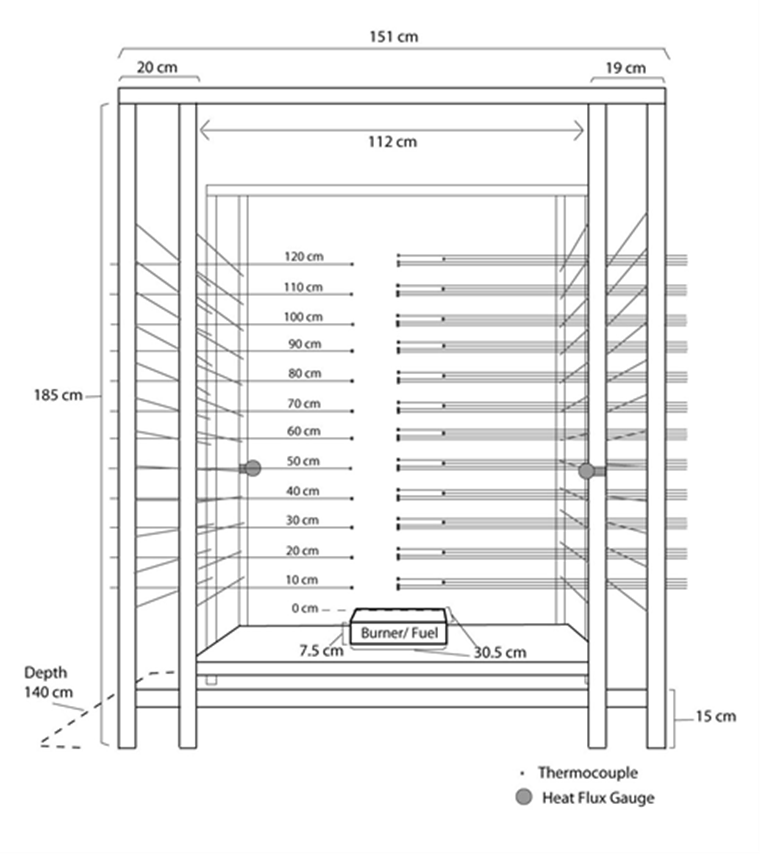
\includegraphics[width=\textwidth]{../Figures/Schematic_Drawing}\\
  \caption[Diagram of the source fire flame and plume instrumentation apparatus]{Diagram of the source fire flame and plume instrumentation apparatus which was centered under the 3~m by 3~m oxygen consumption calorimeter.  The heat flux gauges were facing toward the center of the burner/fuel area.}
  \label{Drawing_Fire_Flamer}
\end{figure}

\begin{figure}
  \centering
  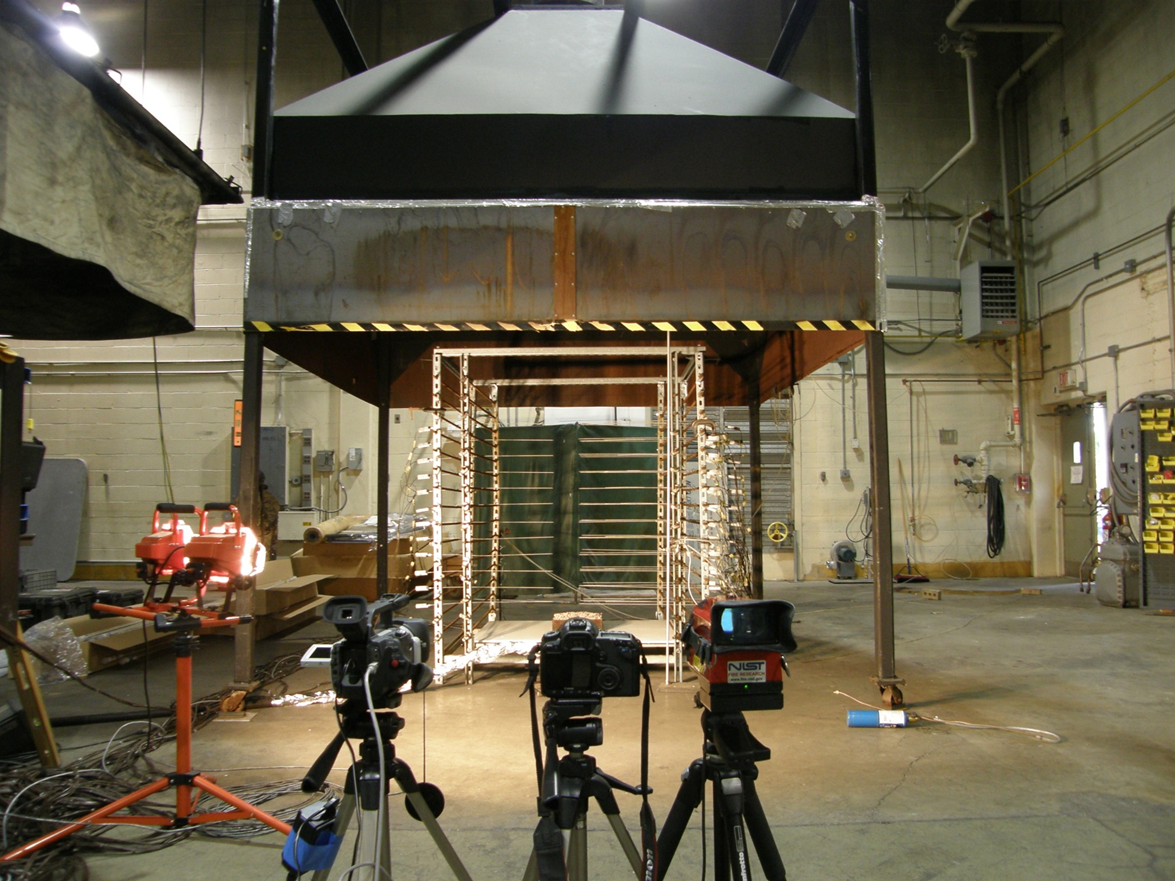
\includegraphics[width=\textwidth]{../Figures/Source_Fire_Flamer}\\
  \caption[A photograph of the source fire flamer and plume instrumentation apparatus]{A photograph of the source fire flamer and plume instrumentation apparatus which was centered under the 3~m by 3~m hood of the oxygen consumption calorimeter.  In the foreground, from left to right, are the video, 35~mm SLR and thermal imaging camera.}
  \label{Fire_Flamer}
\end{figure}



\chapter{Results}
\label{chapter:Results}

{\section{HRR}

Figure~\ref{HRR} shows the measured heat release rates for the natural gas, gasoline and polyurethane foam fueled fires. In each graph, the replicate heat release time histories are overlaid to give a sense of the experimental repeatability for each fuel.

\begin{figure}[p]
  \centering
  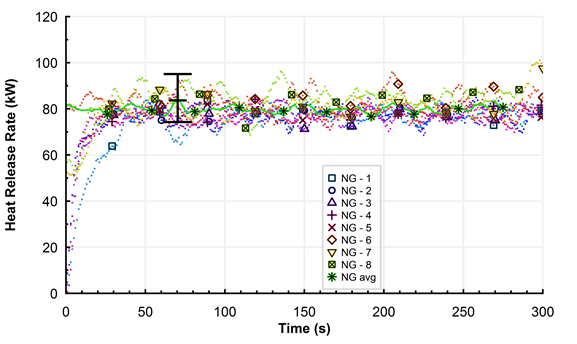
\includegraphics[width=4.5in]{../Figures/Fig3}\\
  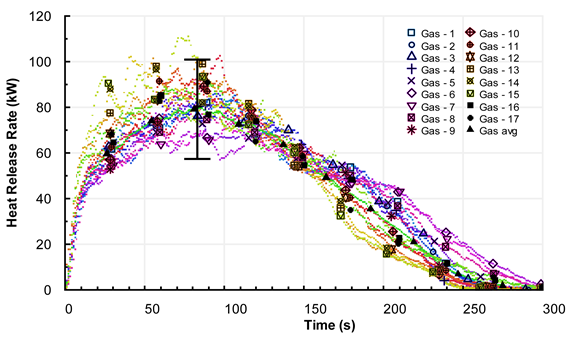
\includegraphics[width=4.5in]{../Figures/Fig4}\\
  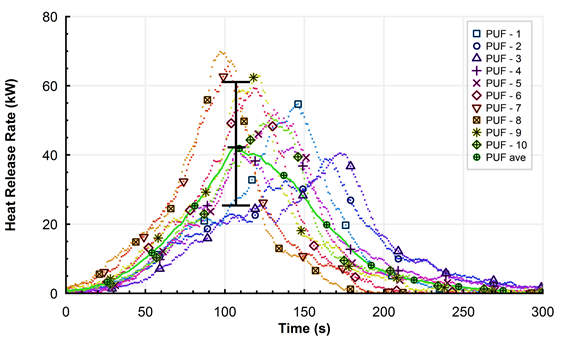
\includegraphics[width=4.5in]{../Figures/Fig5}\\
  \caption[Heat release rates for the natural gas, gasoline and foam fires]{Heat release rates for the natural gas, gasoline, and foam fires.}
  \label{HRR}
\end{figure}

On each fuel’s averaged heat release rate curve, a bar representing the 95~\% confidence level ($2\sigma$), based on Type A evaluation of the uncertainty is provided~\cite{Taylor:1994}.  A Type A evaluation of the uncertainty is any statistical analysis of the data from a series of observations.  In this case the evaluation assumed a normal distribution of the data such that doubling the calculated standard deviation (2σ) would yield a confidence level of approximately 95~\%.

The natural gas burner provided the most repeatable results, with an average steady state heat release rate of 80~kW $\pm$ 9~kW with an average total heat release of 23.3~MJ $\pm$ 1.6~MJ over a 300~s period.  The gasoline, based on the average over a 30 s interval bounding the peak heat release rate of each of the 17 experiments, provided an average peak heat release rate of 80~kW $\pm$ 24~kW.  The total heat release of the gasoline over the 300~s period after ignition was 13.6~MJ $\pm$ 0.6~MJ.  The polyurethane foam demonstrated the largest variability of the three fuels in terms of peak heat release rate and time to peak heat release.  Averaging over a 15~s interval bounding the peak heat release rate from each of the ten experiments yielded an average peak heat release rate of 45~kW $\pm$ 21~kW.  The total heat release over the 300~s period after ignition was 4.1~MJ $\pm$ 0.2~MJ


\section{Plume Temperatures}

Plots of the centerline temperatures averaged over the replicate experiments for each of the fuels are presented in Fig.~\ref{Temp}. The natural gas temperatures were averaged over a ``steady-state'' burning period.  The temperature differences between the vertical thermocouple locations, for locations greater than 20~cm above the fire location, begin to decrease as the distances from the top of the burner increase.  This trend is similar for both the gasoline fires and the polyurethane foam fires as well.  The most notable difference between the natural gas and the other fuels is the growth and decay of the fire during the test period.

\begin{figure}[p]
  \centering
  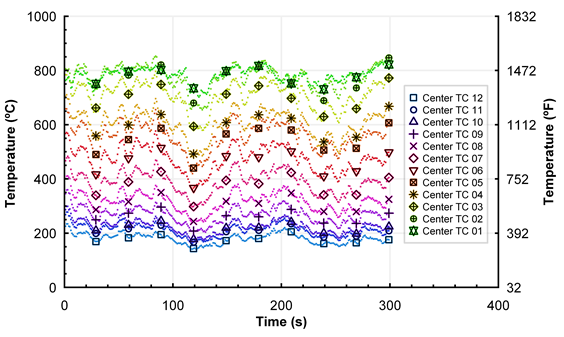
\includegraphics[width=4.5in]{../Figures/Fig6}\\
  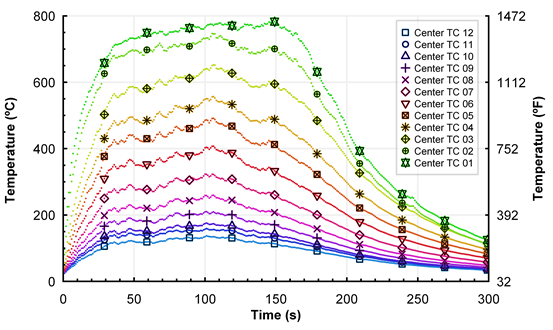
\includegraphics[width=4.5in]{../Figures/Fig7}\\
  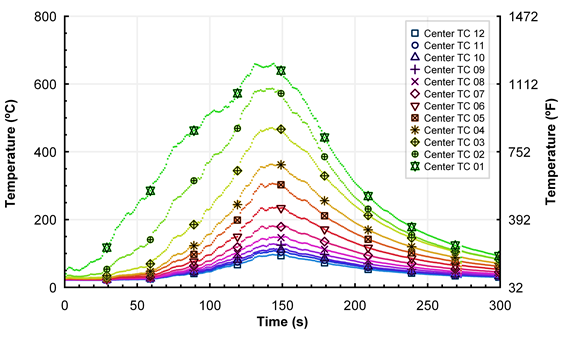
\includegraphics[width=4.5in]{../Figures/Fig8}\\
  \caption[Averaged centerline temperature for the natural gas, gasoline, and foam fires]{Averaged centerline temperature for the natural gas, gasoline, and foam fires. The number following the TC represents the height of thermocouple in decimeters  above the surface of the burner.}
  \label{Temp}
\end{figure}


\section{Total Heat Flux}

Plots of the total heat flux for each of the fuels are presented in Fig.~\ref{Flux}. The repeatability of the total heat flux values varied in a manner similar to the heat release rates, in that the natural gas fires provided a steady state value while the gasoline and the polyurethane foam fires generated a fire curve that has periods of growth and decay.   The sensing surface of the heat flux gauges were located 0.95~m horizontally from the center of the burner/fuel and 0.50~m above the top of the burner/pan lip/fuel surface.  The average peak total heat flux for the natural gas fires were approximately 2.0~kW/m$^2$.  The average peak values for the gasoline and polyurethane foam were approximately 3.5~kW/m$^2$ and 2.5~kW/m$^2$ respectively.  The values are only presented for the experiments which had two heat flux gauges installed as described in the instrumentation section above.

\begin{figure}[p]
  \centering
  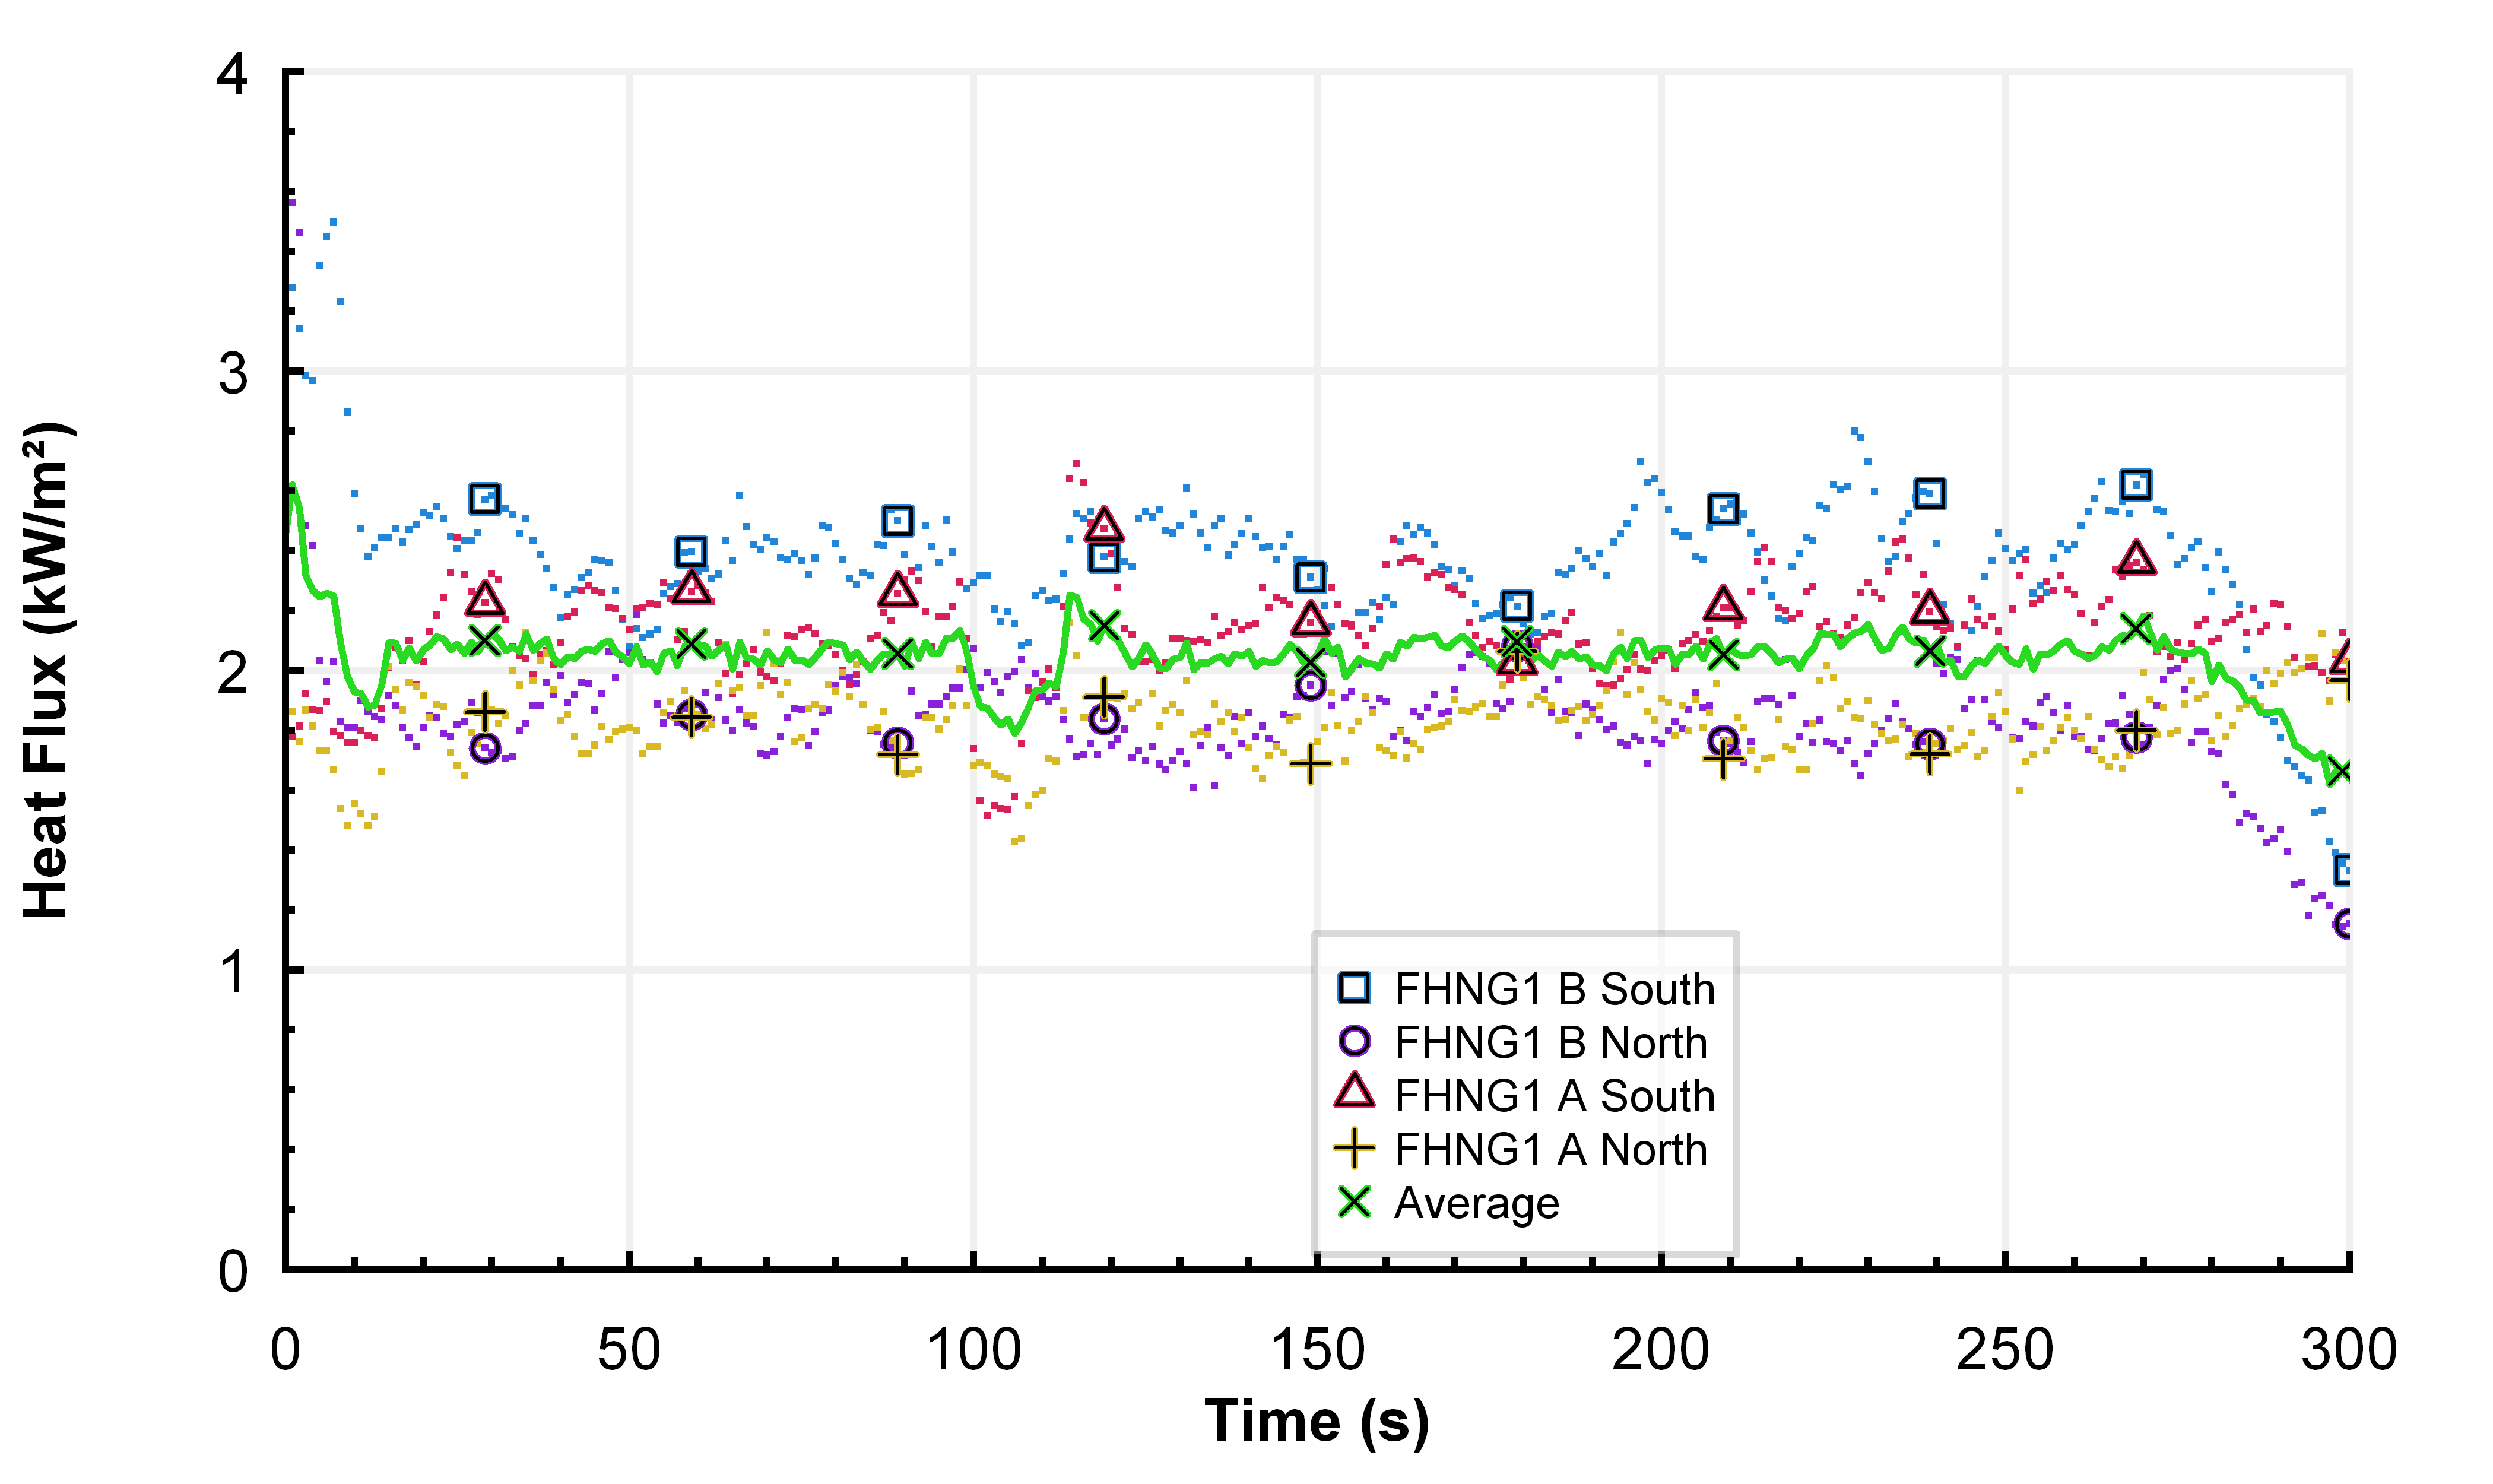
\includegraphics[width=4.5in]{../Figures/Fig9}\\
  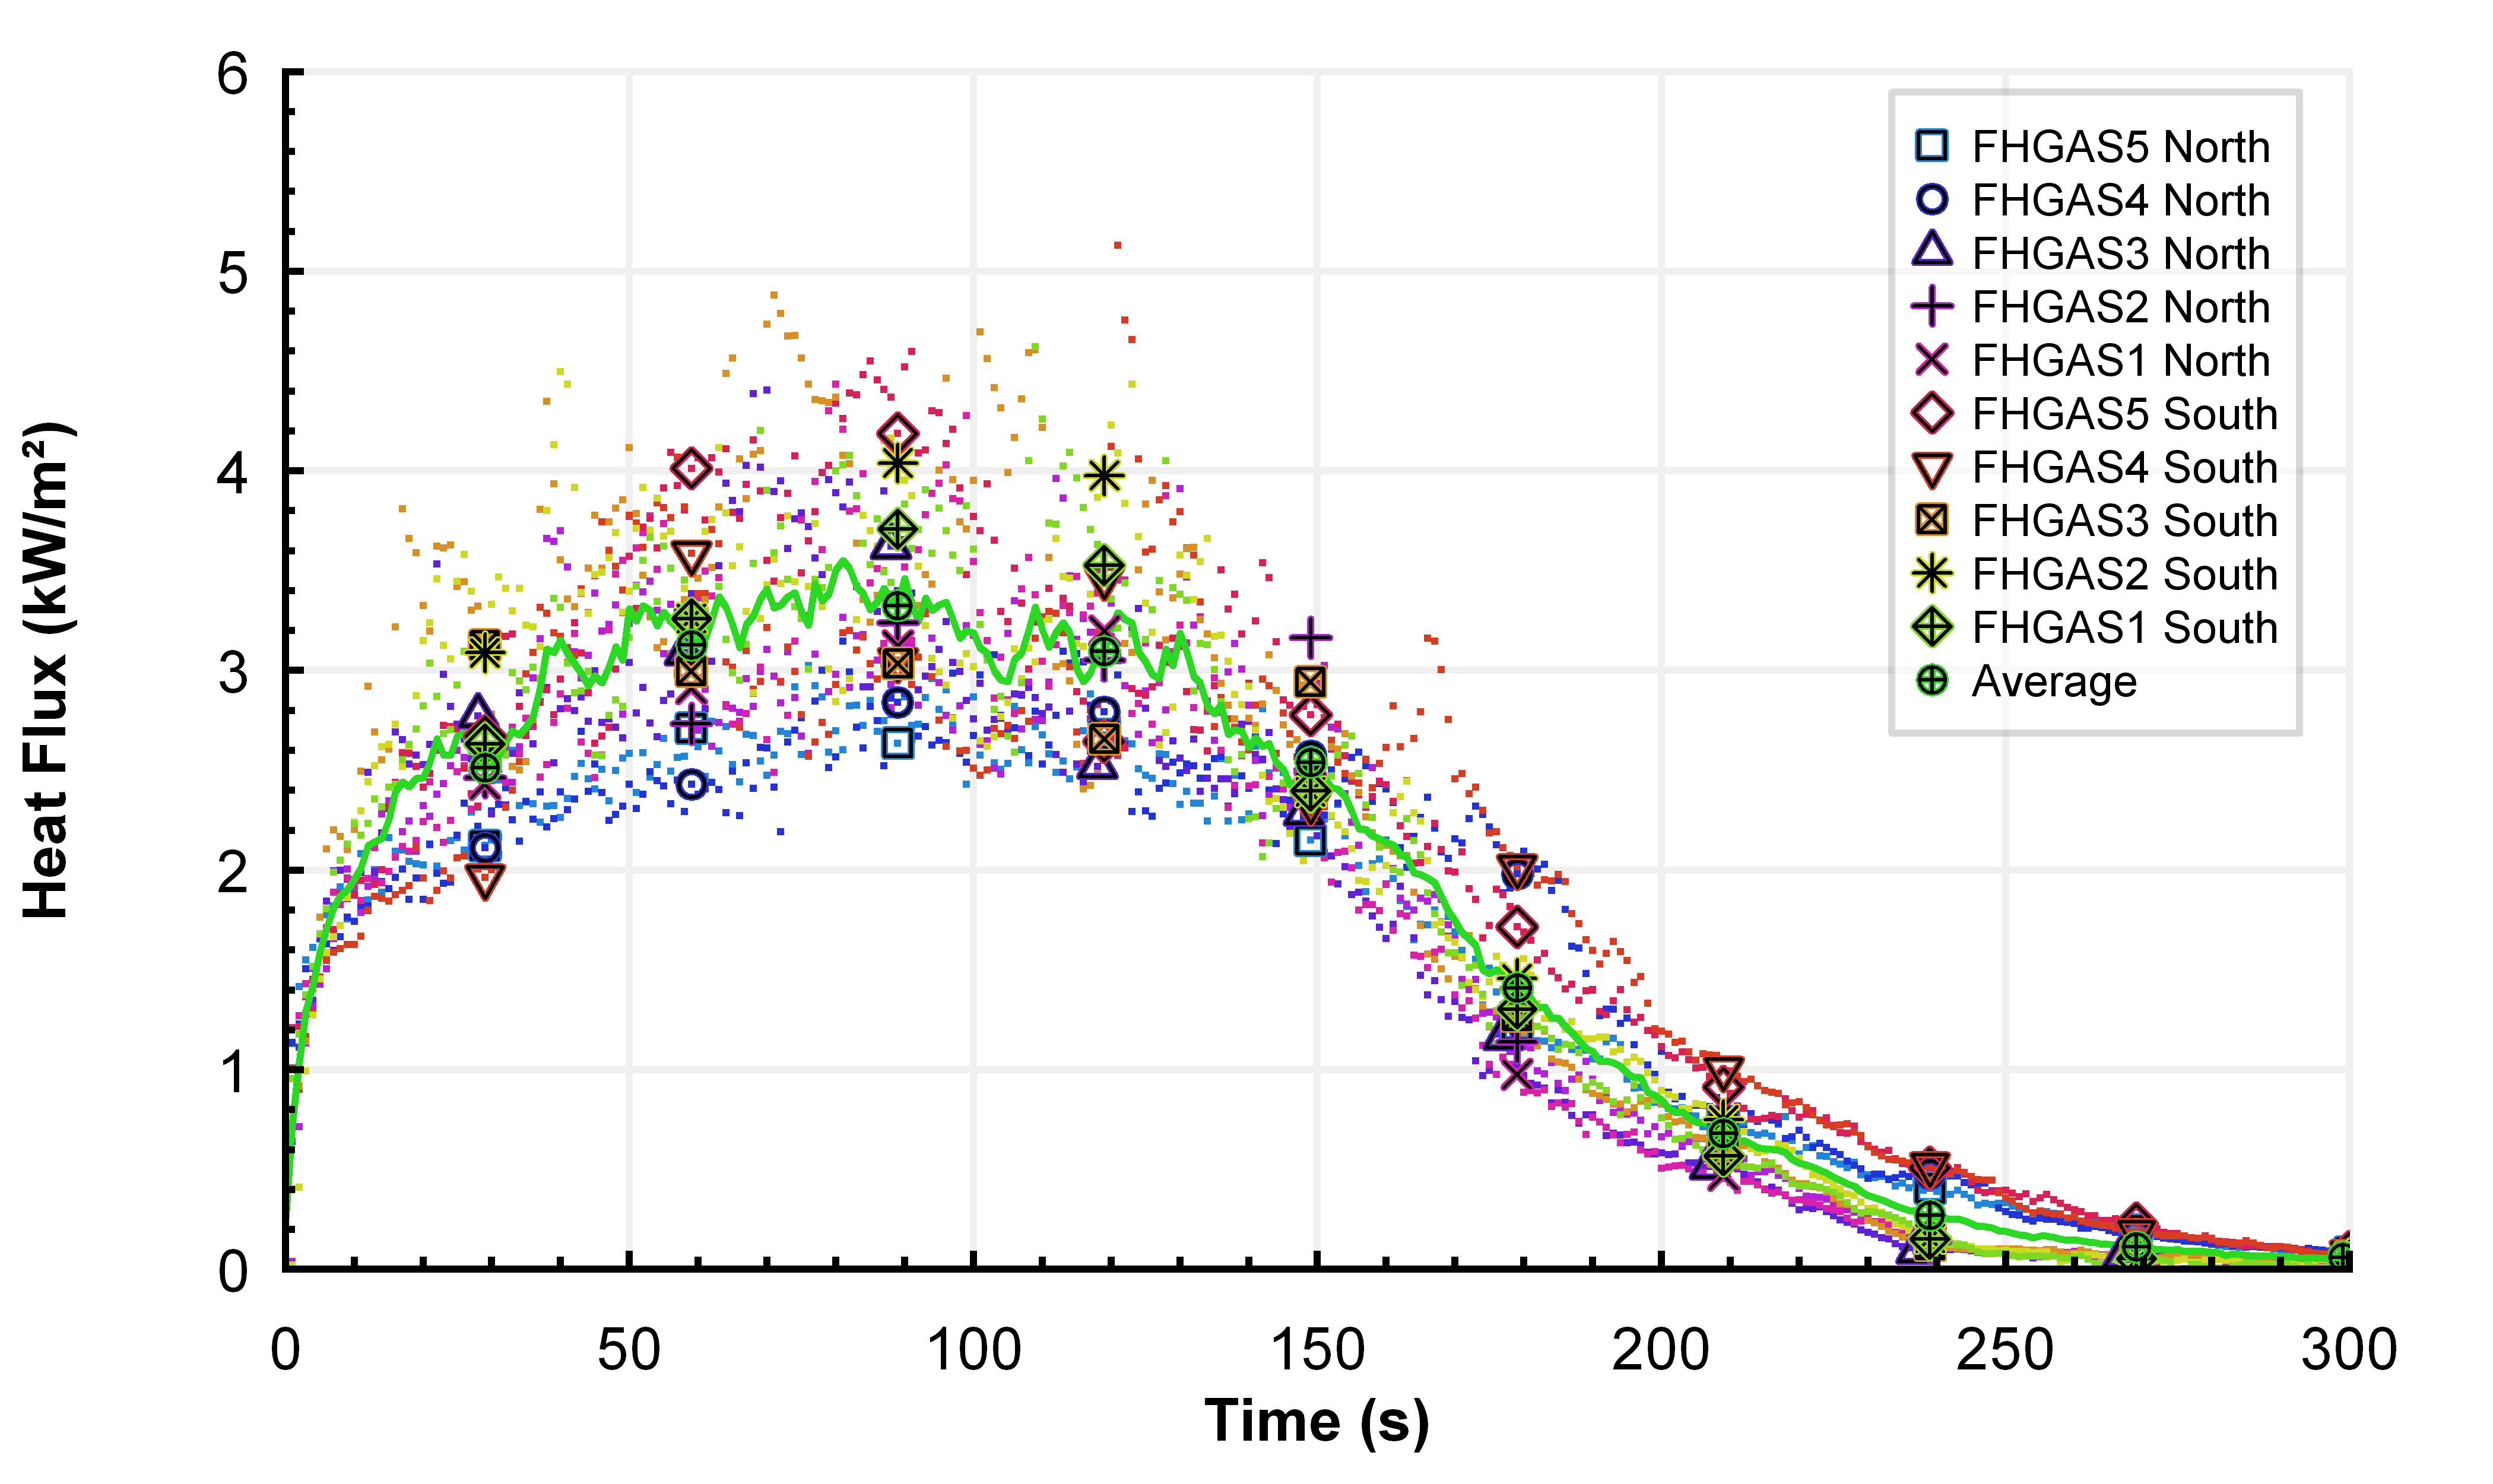
\includegraphics[width=4.5in]{../Figures/Fig10}\\
  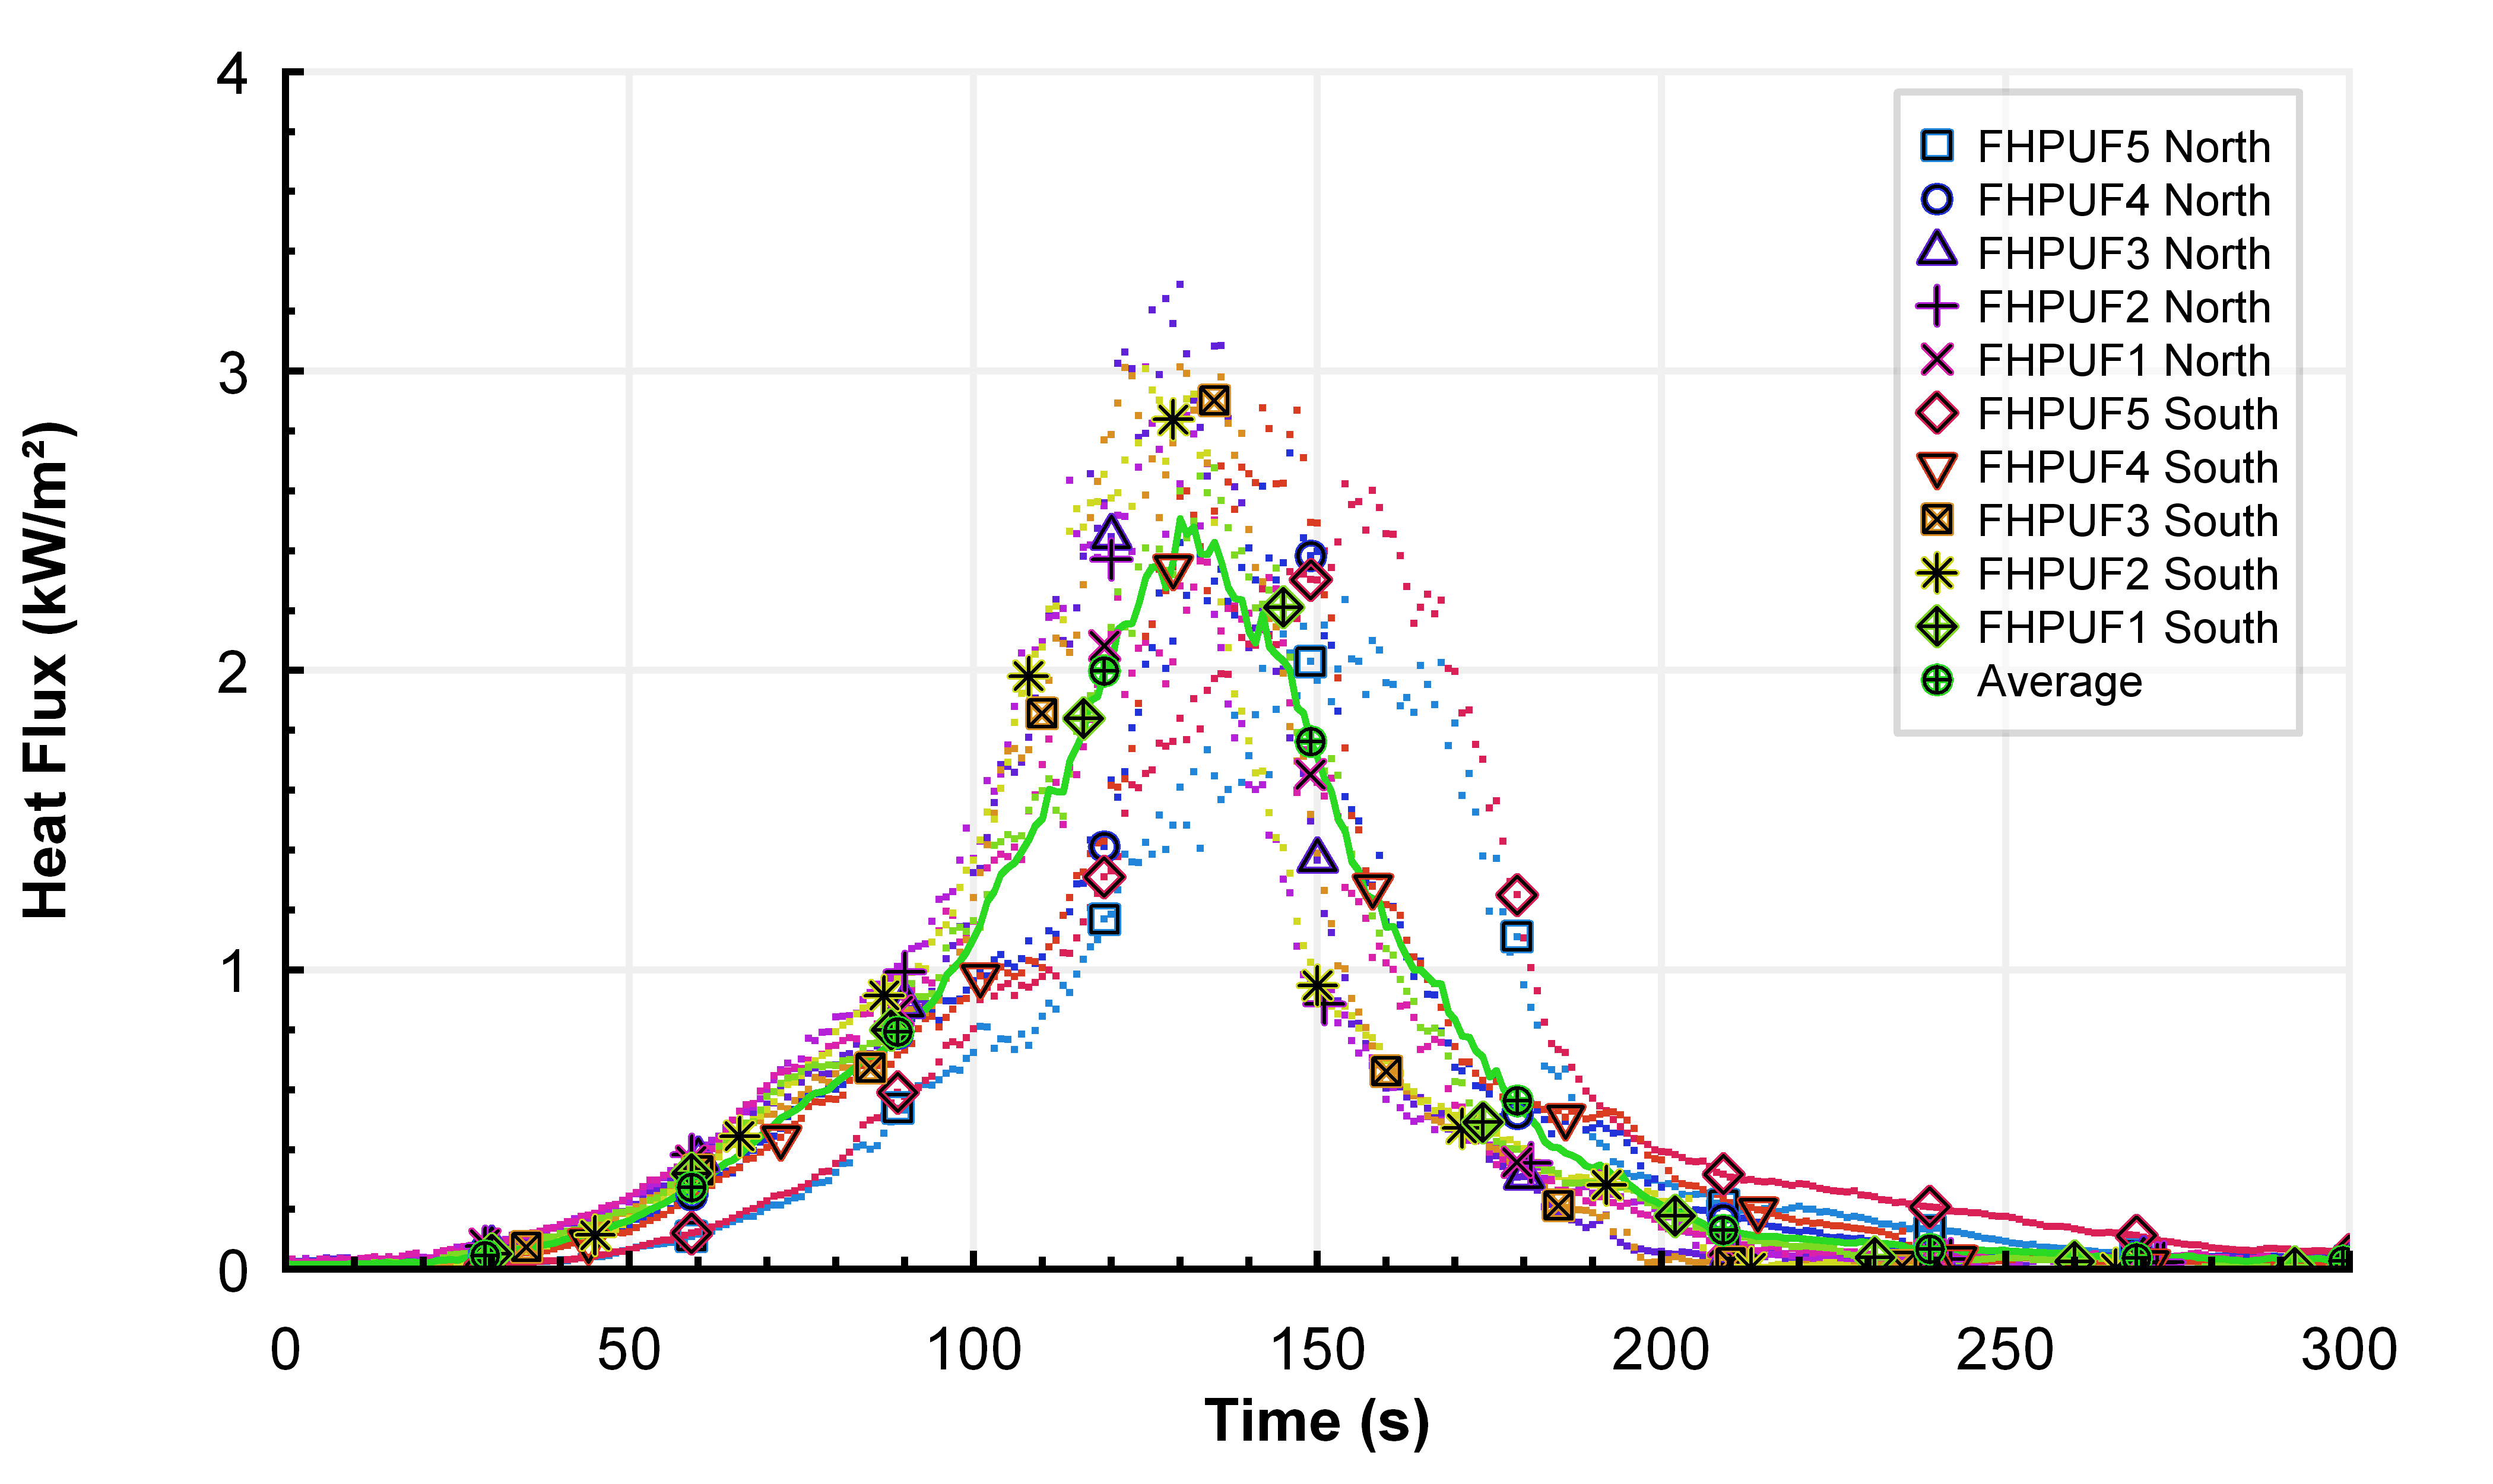
\includegraphics[width=4.5in]{../Figures/Fig11}\\
  \caption[Total heat flux versus time for natural gas, gasoline, and foam fires]{Total heat flux versus time for natural gas, gasoline, and foam fires.}
  \label{Flux}
\end{figure}


\section{Mass Loss}

Mass loss measurements were not possible for the natural gas burner experiments.  The mass loss versus time curves for the gasoline and the polyurethane experiments are shown in Fig.~\ref{Mass}.  The gasoline exhibits a linear mass loss rate for the initial 150~s of approximately 2~g/s.  The polyurethane foam was ignited with a small flame in the center of the top surface of the foam block.  As the flame spread across the surface it also began to burn down into the foam sample.  As a result the exposed surface of the foam began to take the shape of a bowl as the burning rate became linear at approximately 2~g/s.

\begin{figure}[p]
  \centering
  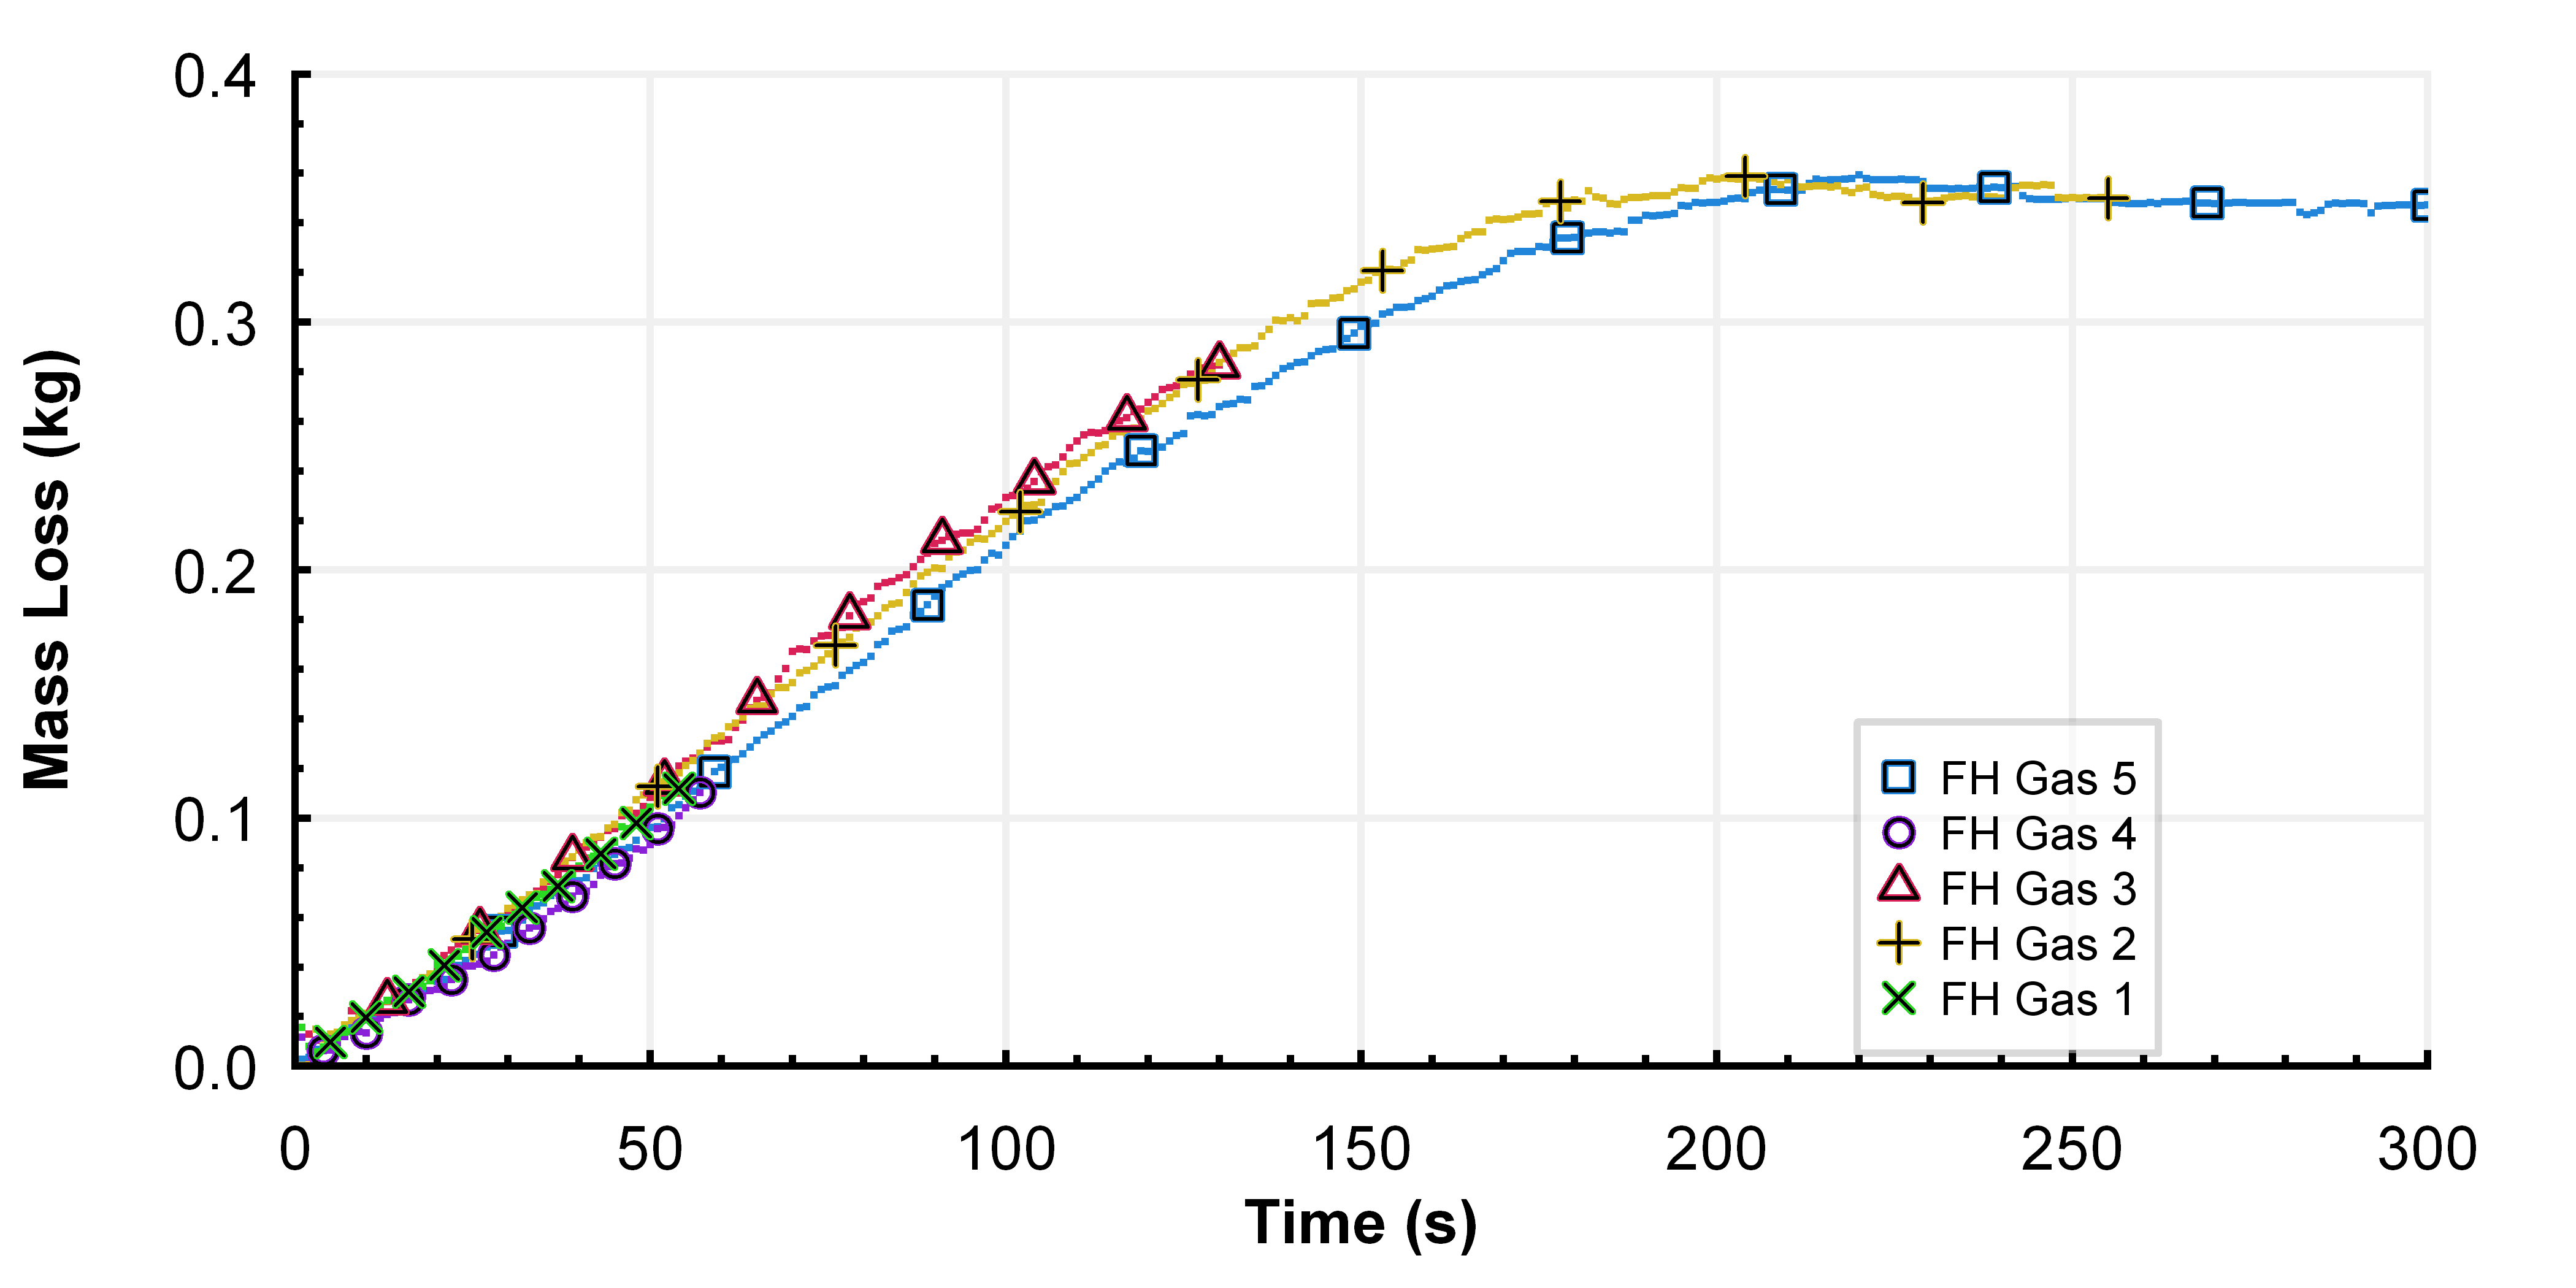
\includegraphics[width=4.5in]{../Figures/Fig12}\\
  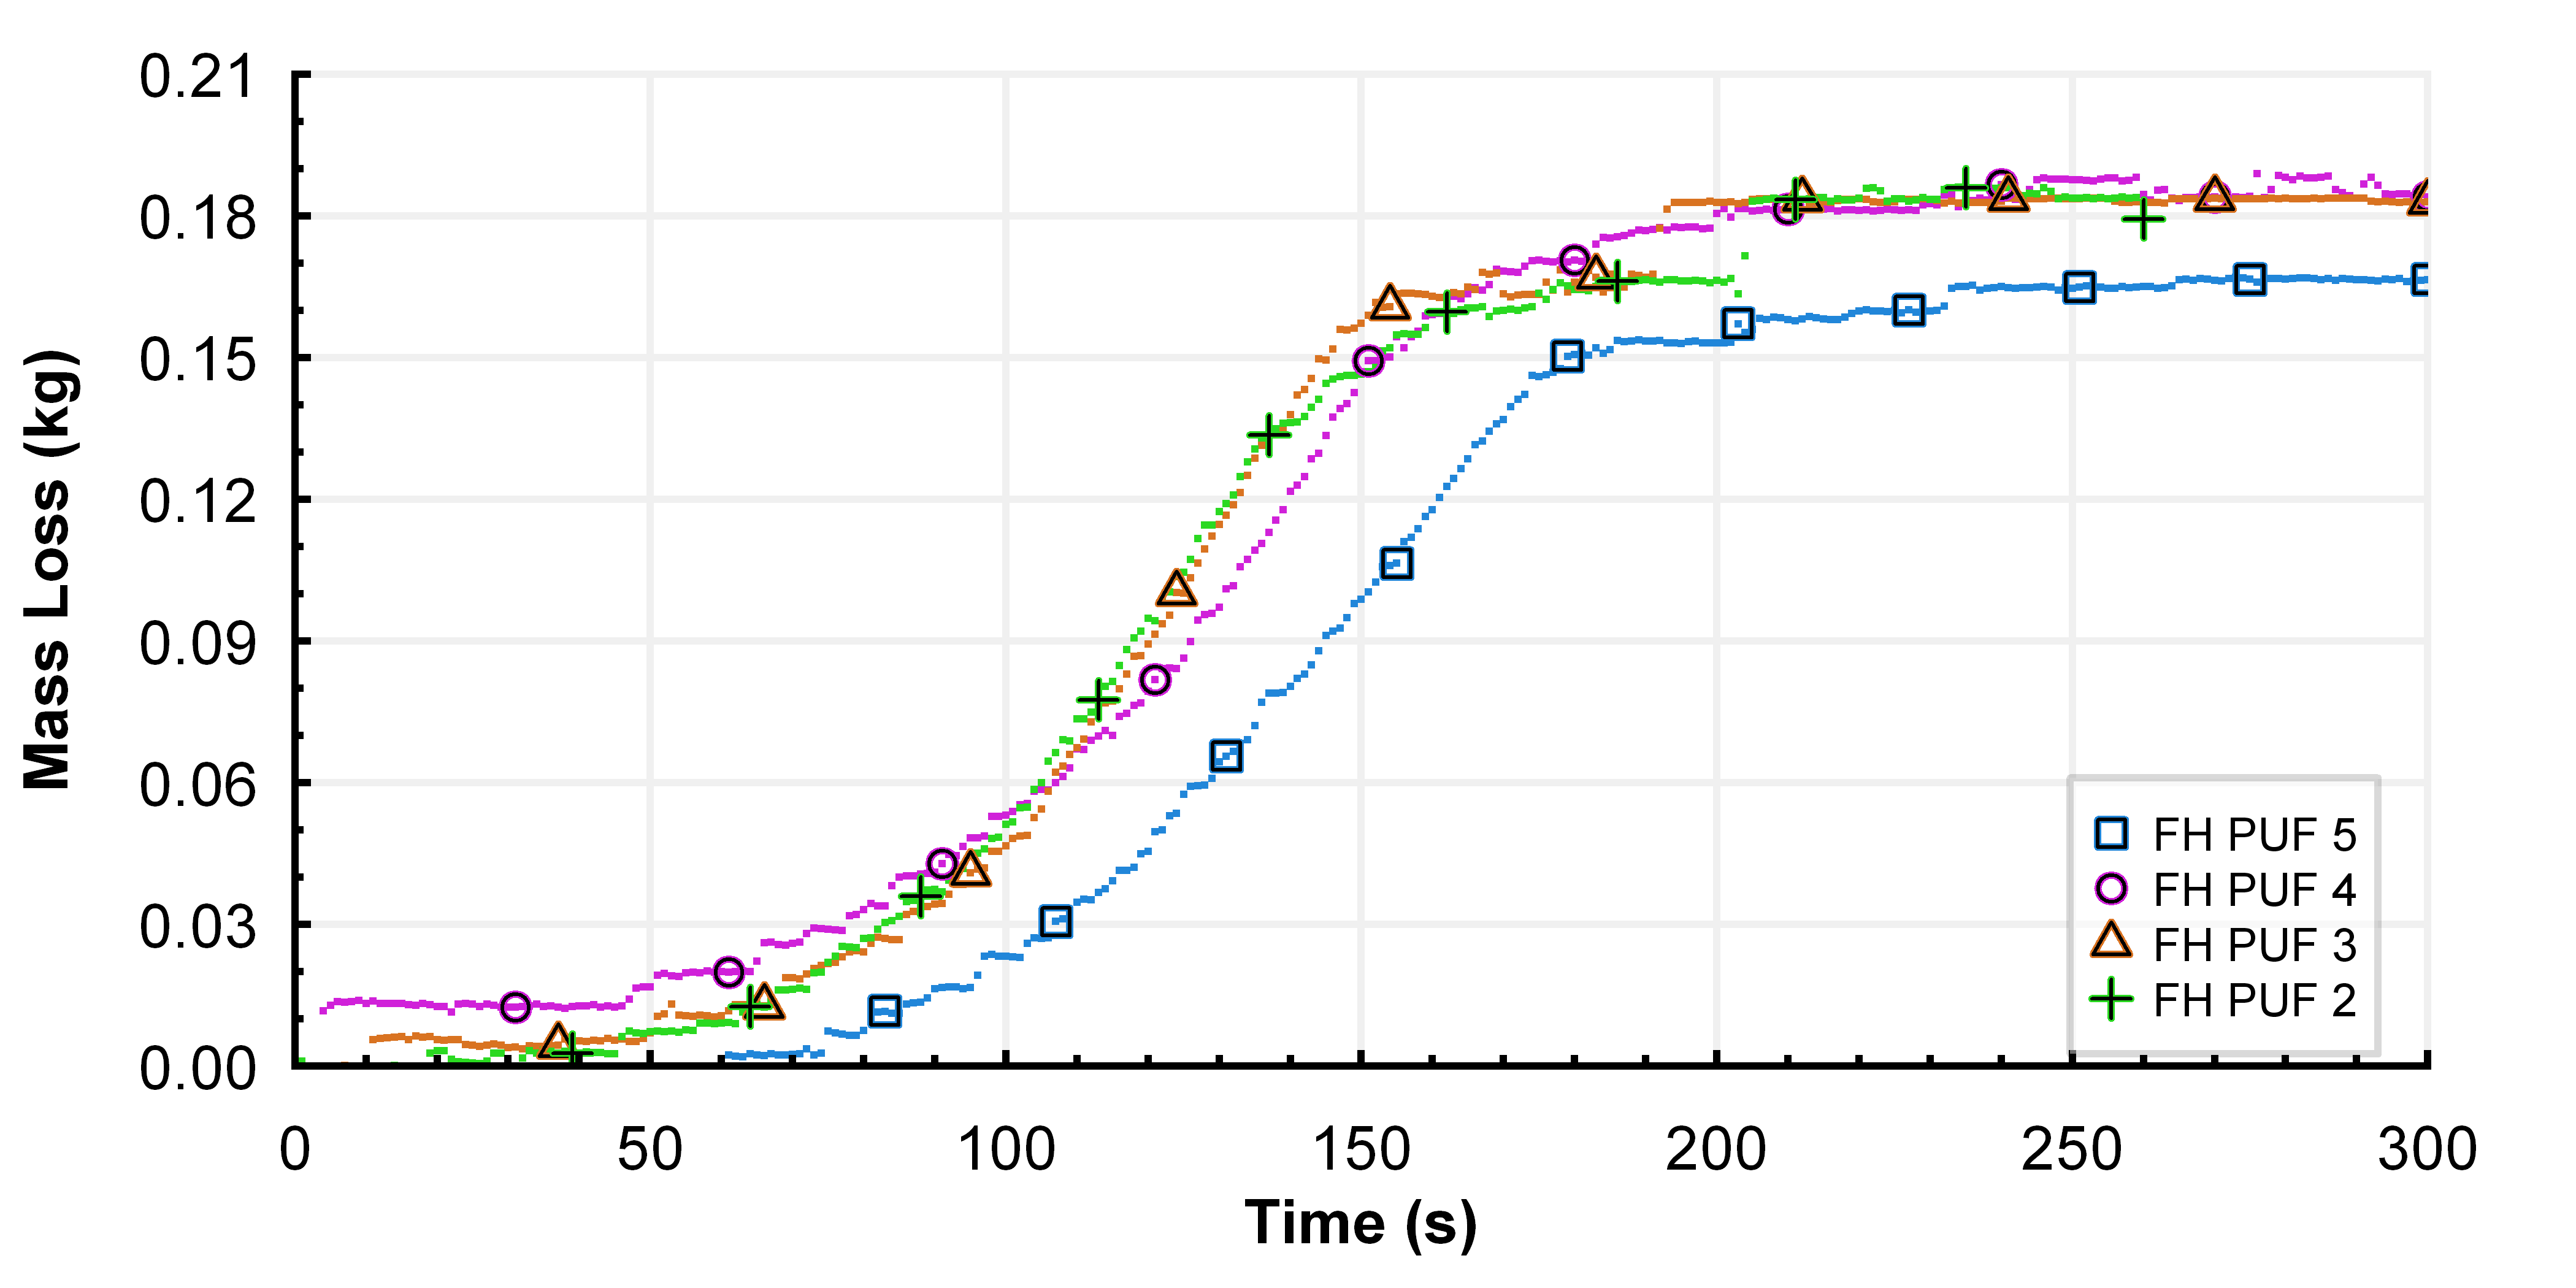
\includegraphics[width=4.5in]{../Figures/Fig13}\\
  \caption[Mass loss versus time for the gasoline and foam fueled fires]{Mass loss versus time for the gasoline and foam fueled fires.}
  \label{Mass}
\end{figure}


\section{Flame Height}

Each of the experiments was photographed with a digital single lens reflex (SLR) camera, fixed on a tripod, with a capability of capturing at least five images per second.  Located adjacent to the camera was a video camera recording images at approximately thirty 30 frames per second (fps).  The experiments were also recorded with a thermal imager, however the videos were not used for analysis as it was difficult to determine the differences between the visible flame and the thermal plume from the black and white images.

In engineering terms, the ``flame height'' is typically discussed as the median flame height.  A position above the top of the fuel surface where the flame is observed to be present at least 50~\% of the time.  As a starting point, the mean flame height for each fuel was estimated from a measurement of the uppermost continuous flame tip from the still photographic images.

Examples of the photographic images are presented in Figs.~\ref{Gas_Foam_Photos} and \ref{Gasoline_Photos}.  Figure~\ref{Gas_Foam_Photos} is a photograph of the natural gas flame taken during a period of ``steady state'' burning at approximately 80~kW and a photograph of the polyurethane foam fire taken near its peak heat release rate of approximately 60~kW.  Figure~\ref{Gasoline_Photos} presents two photographs of the same gasoline fueled fire when it was burning near its peak heat release rate of 100~kW.  The two photographs, taken 0.2~s apart, represent the range of the observed flame heights from one of the gasoline experiments from 0.65~m and 1.0~m, respectively.

\begin{figure}
  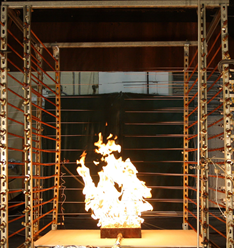
\includegraphics[width=2.7in]{../Figures/Fig14a} 
  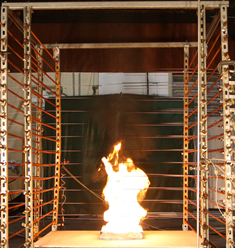
\includegraphics[width=2.7in]{../Figures/Fig14b} \\
  \caption[Photographs of the natural gas and polyurethane foam fires]{Photographs showing a natural gas fire (left) and a polyurethane foam fire (right) under the oxygen consumption calorimeter.}
  \label{Gas_Foam_Photos}
\end{figure}

\begin{figure}
  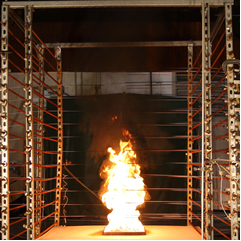
\includegraphics[width=2.7in]{../Figures/Fig15a}
  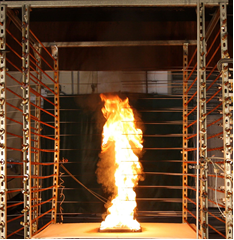
\includegraphics[width=2.7in]{../Figures/Fig15b} \\
  \caption[Photographs of the gasoline fire]{Photograph showing a gasoline fueled experiment with a flame height of 0.65 m (left) and a photograph taken approximately 0.2 s later with a flame height of 1.0 m (right).}
  \label{Gasoline_Photos}
\end{figure}


Table~\ref{tab:Flame_Heights} provides the mean visible flame height, as well as the range of flame heights for each fuel, based on analysis of the photographs for three replicate experiments.  In each case, the photographs were chosen for analysis while the fire was generating its peak heat release rate.  The range of flame heights for each fuel is approximately twice the minimum flame height or the continuous flame height. Analyzing the photographs in this manner was very time consuming and was based on making measurements on each photograph with a scale.  The limit of 5 frames per second also introduces additional uncertainty in determining the flame height. These values will serve as a basis for comparing with mean flame height values determined with video analysis.

As noted by Beyler in his review of fire plume correlations, video tape analysis seems to provide the best estimates of flame height~\cite{Beyler:1986}. Each experiment was recorded with a digital video camera at a refresh rate frequency of 29.97~fps which is the National Television Standards Committee (NTSC) standard. The resulting image in each frame was 720 pixels wide by 480 pixels high. Segments of the video which corresponded to the peak heat release of each experiment were captured with a video editing program.

For the natural gas experiments, approximately 30~s of ``steady state'' video were captured.  In the cases of the gasoline and polyurethane fueled experiments, the video capture period bounded the peak heat release rate.  In the case of the gasoline fueled fires, the peaks occurred over a long period of time, so a 30 s video capture could be made which was representative of the peak burning rate.  The peak duration for the polyurethane foam fires was shorter so, only a 15~s video capture was used.

\begin{table}
  \centering
  \begin{tabular}{|l|c|c|}
     \hline
     Fuel	            & Mean (m)  & Range (m) \\ \hline
     Natural Gas	    & 0.70	    & 0.50 to 0.98 \\
     Gasoline 	        & 0.84	    & 0.52 to 1.10 \\
     Polyurethane Foam  & 0.46	    & 0.30 to 0.78 \\
     \hline
   \end{tabular}
  \caption[Mean visible flame height and averaged minimums and maximums]{Mean visible flame height and averaged minimums and maximums (Range) of visible flame heights for each of the fuels during peak heat release rate.}
  \label{tab:Flame_Heights}
\end{table}

Each frame from the video clip was saved as a full color Tagged Image File Format (TIFF) file and the pixel aspect ratio was changed from 0.9 to 1, so that each pixel had the same dimension in both the horizontal and vertical directions.  Once these images were rendered by the video editing program, each image was scaled and cropped to provide input for Streams, a suite of image processing programs developed by Nokes for analyzing fluid flow visualization experiments~\cite{Nokes:2011}. The images were scaled so that one pixel equals 5~mm in height and width.

Examples of a set of TIFF images for each fuel are shown in Figures~\ref{flame_height_comp_FHNG80_1} through \ref{flame_height_comp_FHPUF_1}.   Each figure has 56 sequential images from the video segment.  The images total almost 2~s of actual burn time.  Notice how the flame height cycles up and down in each of the sequences.  These images provide additional information and continuity of the motion of the flame so that the analysis is less likely to miss and extreme (minimum or maximum) position when compared to the still photographs.
\begin{figure}
	\centering
	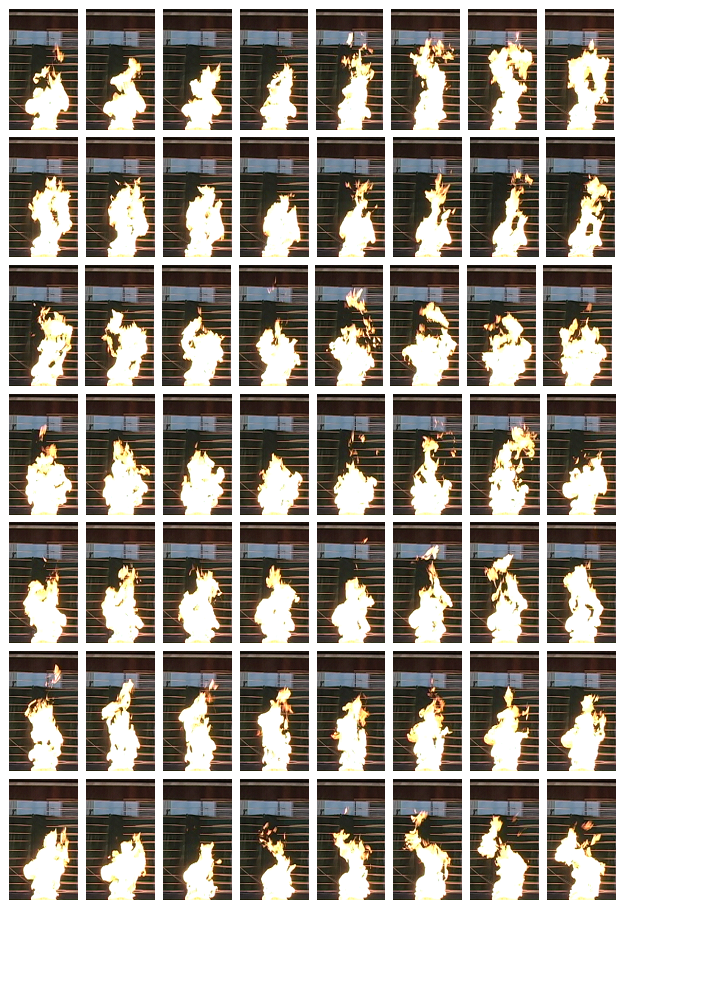
\includegraphics[width=\textwidth]{../Figures/flame_height_comp_FHNG80}\\
	\caption[Example of sequential video frames sampled from a natural gas fueled experiment]{Example of sequential video frames sampled from a natural gas fueled experiment.  In this set of images, which spans almost two seconds, the visual continuous flame height fluctuates from approximately 0.6 m to 1.1 m.}
	\label{flame_height_comp_FHNG80_1}
\end{figure}

\begin{figure}
	\centering
	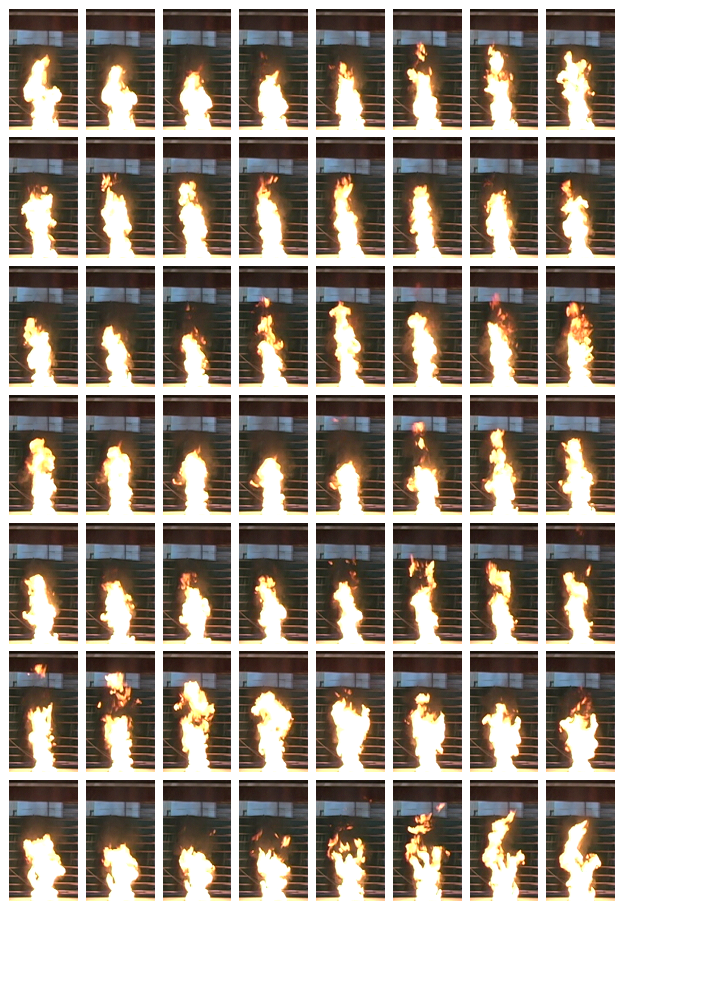
\includegraphics[width=\textwidth]{../Figures/flame_height_comp_FHGAS}\\
	\caption[Example of sequential video frames sampled from a gasoline fueled experiment]{Example of sequential video frames sampled from a gasoline fueled experiment.  In this set of images which spans almost two seconds the visual continuous flame height fluctuates from approximately 0.6 m to 1.1 m.}
	\label{flame_height_comp_FHGAS_1}
\end{figure}

\begin{figure}
	\centering
	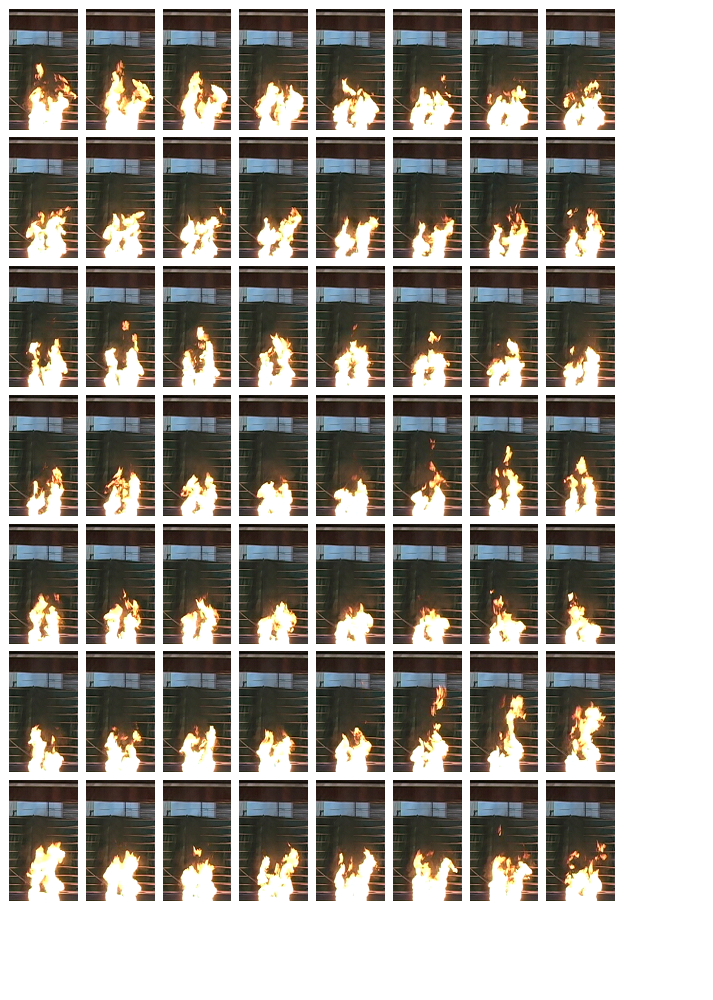
\includegraphics[width=\textwidth]{../Figures/flame_height_comp_FHPUF}\\
	\caption[Example of sequential video frames sampled from a polyurethane foam fueled experiment]{Example of sequential video frames sampled from a polyurethane foam fueled experiment.  In this set of images which spans almost two seconds the continuous visual flame height fluctuates from 0.4 m to 0.9 m.}
	\label{flame_height_comp_FHPUF_1}
\end{figure}


From each of the peak heat release rate video clips, the edited TIFF files were loaded into Streams~\cite{Nokes:2011}.  For the natural gas and gasoline fueled fires, approximately 900 images were used in each image sequence.  The polyurethane foam experiments had approximately 450 images in each sequence for each experiment.  Once the image sequence was created, a series of filters and amplifiers are applied to the images to eliminate all colors but red, based on a method developed by Goble~\cite{Goble:2007}.  Once all of the images were converted to a pure red ``flame'' which represented the area of visible fire, on a black background, the images were processed within Streams to develop an intensity field based on all of the images being ``overlaid'' on each other.  The end result is a contour plot of the intermittency of the flame ranging from zero to one.

The calculations for the intensity field are based on a user defined computation grid.  A grid sensitivity analysis was conducted with 5~mm, 10~mm, 20~mm, 40~mm and 80~mm square grids.  Examples of grid cell resolution outputs from Streams for the natural gas fueled burner are shown in Fig.~\ref{Intensity}.  The outputs shown are time averaged intensity fields generated with 5 resolutions listed above. In each output the x and y axis dimensions are in mm.

\begin{figure}[p]
	\centering
	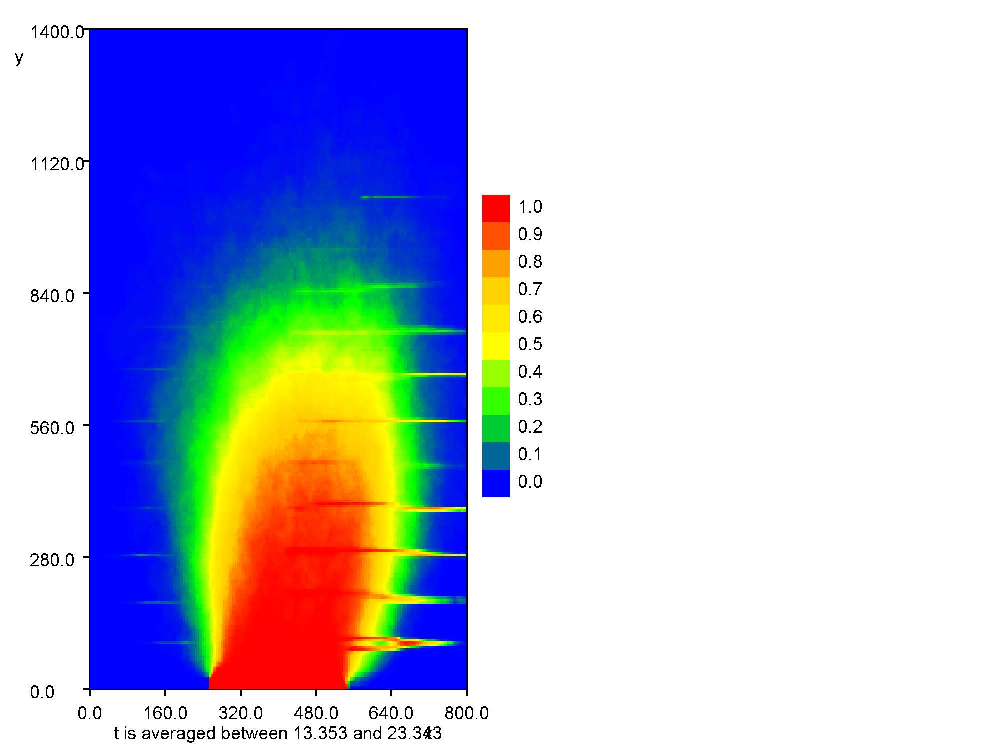
\includegraphics[trim=0in 0in 3.5in 0in,clip=true,width=1.7in]{../Figures/FHNG80-1_GS_5mm_10s_color}
	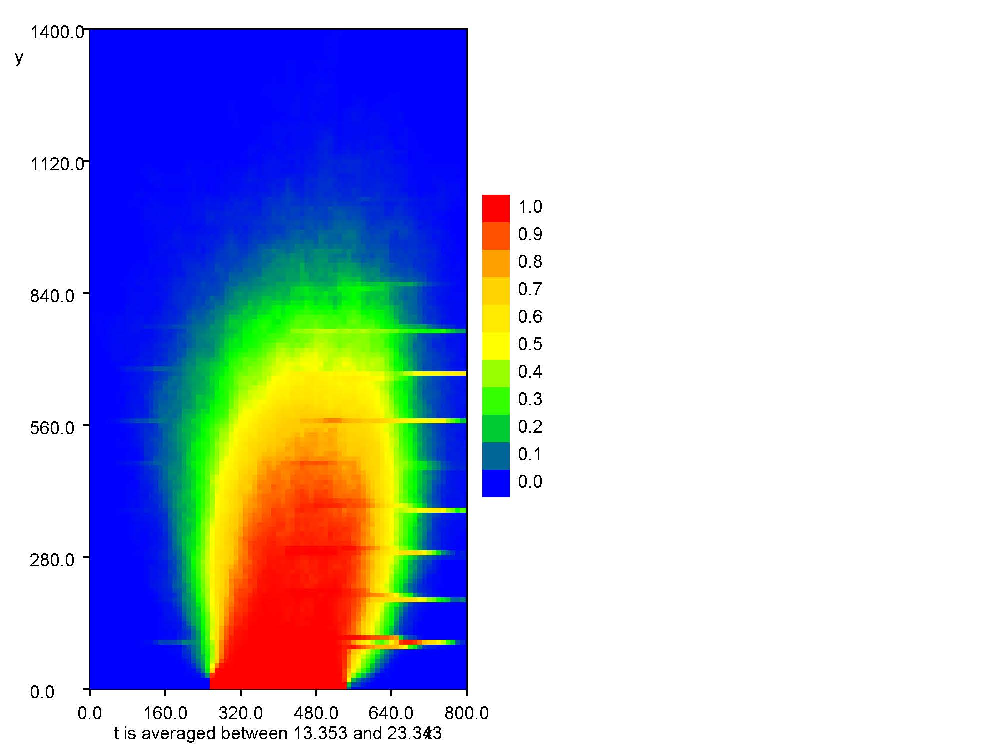
\includegraphics[trim=0in 0in 3.5in 0in,clip=true,width=1.7in]{../Figures/FHNG80-1_GS_10mm_10s_color}\\
	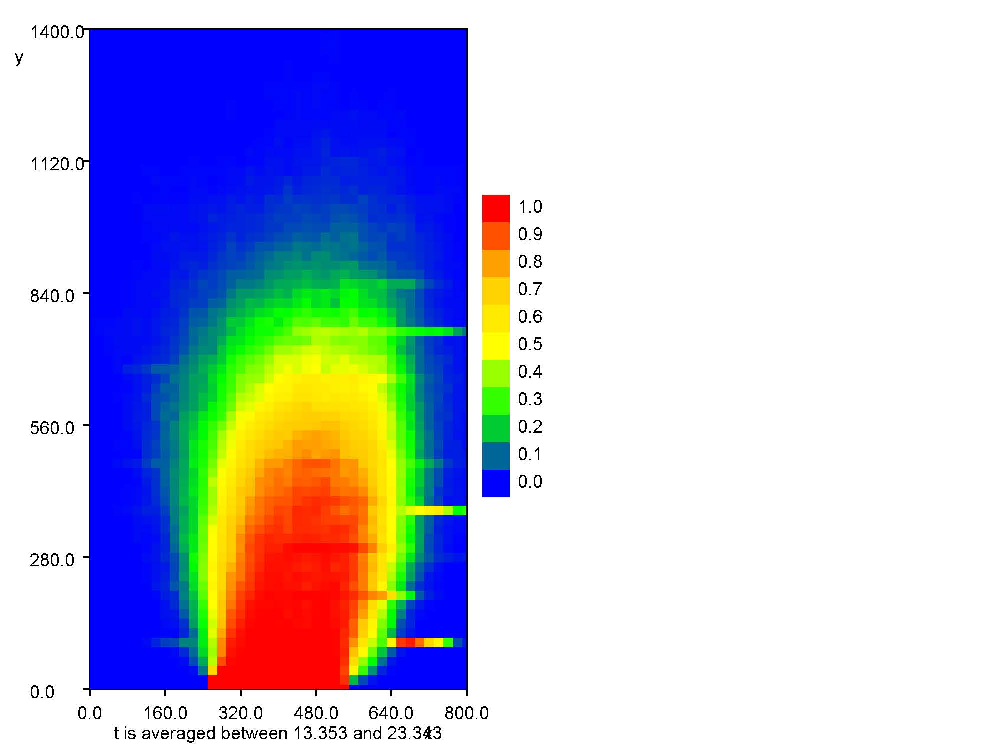
\includegraphics[trim=0in 0in 3.5in 0in,clip=true,width=1.7in]{../Figures/FHNG80-1_GS_20mm_10s_color}
	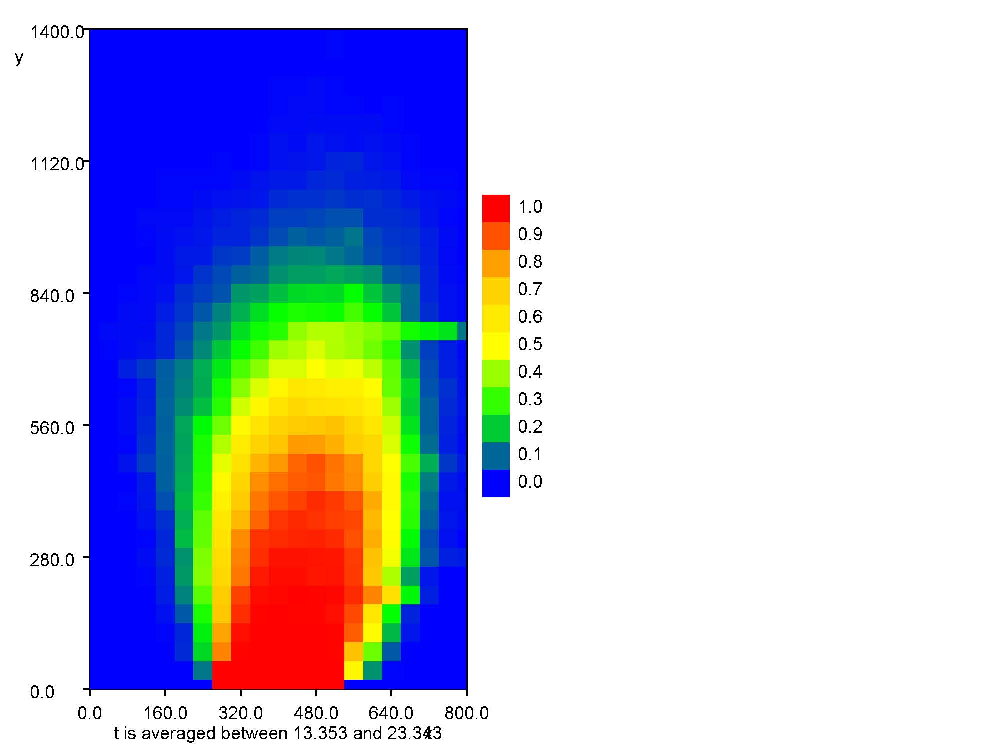
\includegraphics[trim=0in 0in 3.5in 0in,clip=true,width=1.7in]{../Figures/FHNG80-1_GS_40mm_10s_color}
	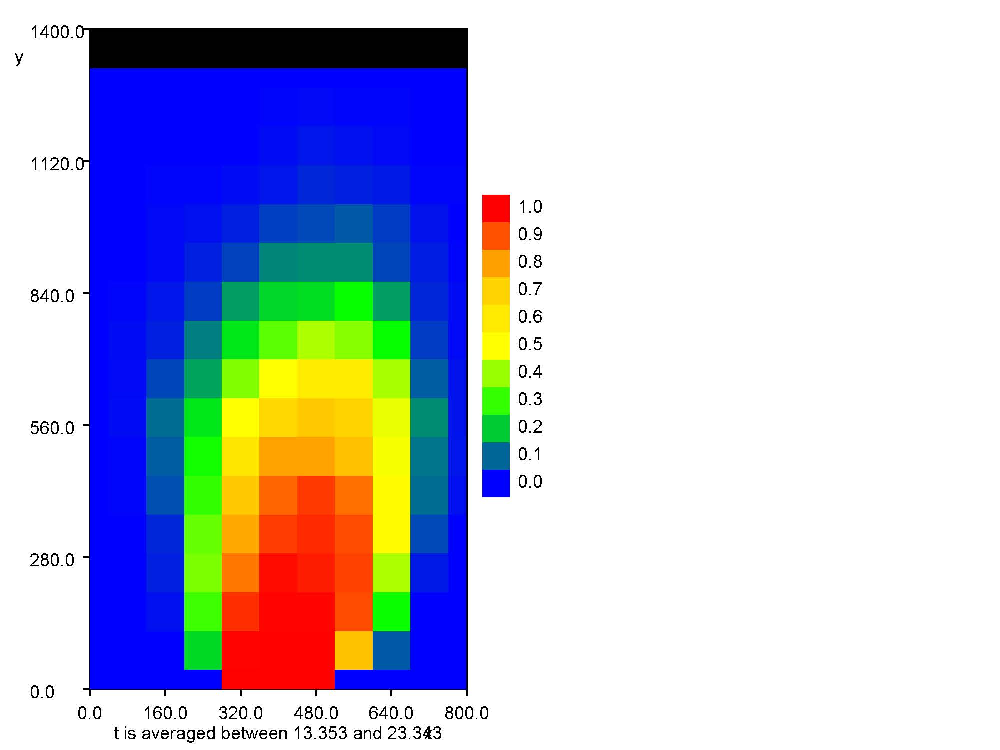
\includegraphics[trim=0in 0in 3.5in 0in,clip=true,width=1.7in]{../Figures/FHNG80-1_GS_80mm_10s_color}\\
	 \caption[Comparison images of intensity fields derived from the video images of the natural gas fueled fire]{Comparison images of intensity fields derived from the video images of the natural gas fueled fire using Streams. The images, starting with the upper left, were generated with 5 mm, 10 mm, 20 mm, 40 mm and 80 mm resolutions.}
	 \label{Intensity}
\end{figure}


Since each pixel in the original images was equal to 5~mm, in the highest resolution case, the 5~mm analysis grid would match the best resolution of the original image.  Four of the five cases resulted in similar results, only the 80~mm case generated significantly different results in flame height.  As a result of the sensitivity analysis, a 10~mm grid was chosen as an optimum size for providing a sufficient level of resolution, enabling efficient processing of 30~s worth of video frames.  At the 5~mm grid resolution, limitations within the processing system would not allow a full 30~s of video analysis.  Therefore the intensity fields and the resulting plots and data generated for this study were developed with a 10~mm grid.

Another means of quantifying field data with Streams is the use of contour plots.  Examples of the time averaged contour plots are shown in Figs.~\ref{Gas_and_Gasoline_Contours} and \ref{Foam_Contours} for the natural gas, gasoline, and polyurethane fueled fires.  Each contour line represents the percentage of time that the flame was at a given position. The region under examination, as shown as a black bounding rectangle, is 1400~mm high and 800~mm in width.  The natural gas fire was sampled for 29~s, resulting in 870~images. The area bounded by the contour with the value 1 represents the area that the flame was visible 100~\% of the time sampled. This can be considered the persistent flame region as defined by McCaffrey~\cite{McCaffrey:1979}. The remaining contours are in the intermittent flame region, with the 0.5 contour representing the mean flame height. Outside of the final contour, value 0.0, no visible flame was recorded; hence this contour marks the definitive start of the buoyant plume region.

\begin{figure}
  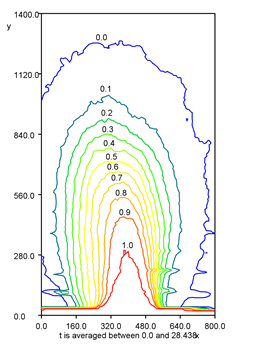
\includegraphics[width=2.7in]{../Figures/Fig20} 
  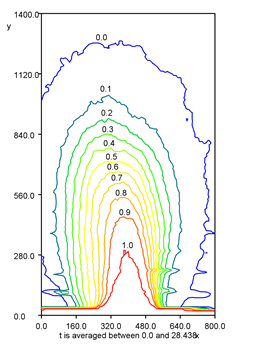
\includegraphics[width=2.7in]{../Figures/Fig21} \\
  \caption[Visibility fractions for the natural gas and gasoline fires]{Plots showing the fraction of time that the flame was visible for the natural gas (left) and gasoline (right) fires.}
  \label{Gas_and_Gasoline_Contours}
\end{figure}

\begin{figure}
  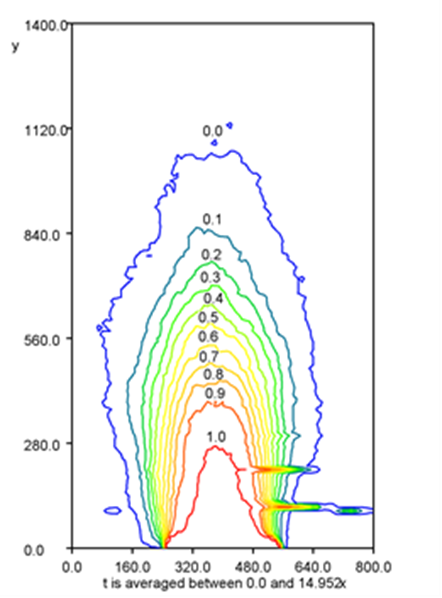
\includegraphics[width=2.7in]{../Figures/Fig22} 
  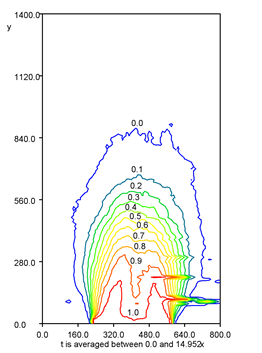
\includegraphics[width=2.7in]{../Figures/Fig23} \\
  \caption[Visibility fractions for the polyurethane foam fire]{(Left) Plot showing the fraction of time that the flame was visible for the polyurethane foam fire. (Right) Polyurethane foam contour plot with bifurcated flames at time of peak heat release rate.}
  \label{Foam_Contours}
\end{figure}

Figure~\ref{Foam_Contours} shows two different contours for the polyurethane foam fueled experiment.  The results from polyurethane fueled fire characterization experiments have an increased amount of variability due to the nature of the ignition source and the fuel itself.  The polyurethane foam was readily ignited with a small pilot flame similar to that used to ignite the natural gas and the gasoline.  By comparison, a small flame ignited the gases flowing out the top of the natural gas burner and the flames from the natural gas cover entire burner surface within approximately one second.  A similar ignition sequence occurs with the gasoline pan fires. The polyurethane foam has a more complicated flame spread sequence that resulted in significant changes to the peak heat release rate and the time to peak heat release.  Once the polyurethane foam was ignited, it took approximately 60~s for the flame to spread across the top surface of the fuel.  As the flames spread horizontally across the fuel surface, the fire also burns down into the fuel.  In some cases the fire burned completely through the fuel in the center of the foam sample, resulting in a hollow flame at the time of the peak heat release rate.  An example of a contour plot, exhibiting the hollow or bifurcated flames is shown at right in Fig.~\ref{Foam_Contours}.  Other methods of ignition for the polyurethane foam were considered in order to have a more uniform ignition of the top surface of the foam.  Each method would have resulted in a larger release of energy from the ignition source or a starter fuel.   Based on a few scoping experiments these methods did not improve the repeatability.

Based on the field data developed using Streams average flame heights for each fuel were determined.  In Table~\ref{tab:Average_Flame_Heights}, each of the values represents the average flame heights, given in mm with 95~\% confidence limits based on a Type A statistical analysis of the data, for each of the source fuels shown as the percentage of time the flame was visible at that given height.  For the natural gas fires, the averages are from ten 30 s segments, while the fire was monitored at approximately 80~kW.  In some cases more than one 30 s segment was sampled per heat release rate experiment.  Sixteen 30~s video segments, which included the peak heat release rate, were successfully analyzed from the seventeen gasoline heat release rate experiments.  One of the videos was unusable for analysis due to reflected light which could not be edited out of the images.  For same reason, the polyurethane foam flame height averages are the result from eight of the ten heat release rate experiments.

\begin{table}
\centering
\begin{tabular}{|c|c|c|c|}
\hline
Visible         &   \multicolumn{3}{|c|}{Visible Flame Heights (mm)} \\ \cline{2-4}
Fraction (\%)   &       Natural Gas	            &   Gasoline	            & Polyurethane Foam \\ \hline
10              &       980 $\pm$ 155 (16~\%)   &	930 $\pm$ 130 (14~\%) 	& 650 $\pm$ 220 (34~\%)   \\
20              &   	890 $\pm$ 125 (14~\%)   &	850 $\pm$ 120 (14~\%) 	& 590 $\pm$ 190 (32~\%)   \\
30              &   	820 $\pm$ 125 (15~\%)   &	790 $\pm$ 110 (14~\%) 	& 540 $\pm$ 180 (33~\%)   \\
40              &   	760 $\pm$ 105 (14~\%)   &	740 $\pm$ 95 (13~\%) 	& 500 $\pm$ 165 (33~\%)   \\
50              &   	705 $\pm$ 106 (15~\%)   &	695 $\pm$ 95 (14~\%) 	& 470 $\pm$ 160 (34~\%)   \\
60              &   	650 $\pm$ 100 (15~\%)   &	655 $\pm$ 85 (13~\%) 	& 435 $\pm$ 135 (31~\%)   \\
70              &   	590 $\pm$ 90 (15~\%)    &	610 $\pm$ 90 (15~\%) 	& 400 $\pm$ 125 (31~\%)   \\
80              &   	530 $\pm$ 85 (16~\%)    &	555 $\pm$ 90 (16~\%) 	& 360 $\pm$ 110 (31~\%)   \\
90              &   	440 $\pm$ 75 (17~\%)    &	490 $\pm$ 95 (19~\%) 	& 315 $\pm$ 110 (35~\%)   \\
100	            &       220 $\pm$ 84 (38~\%)    &	350 $\pm$ 110 (32~\%) 	& 210 $\pm$ 125 (60~\%)   \\
\hline
\end{tabular}
 \caption[Average flame heights for three fuels]{Average flame heights with 95~\% confidence limits, for each of the source fuels shown as the percentage of time the flame was visible at that given height.}
 \label{tab:Average_Flame_Heights}
\end{table}


For both the natural gas and the gasoline experiments the 95~\% confidence limits show less than 20 percent variation in visible flame height within the intermittent flame region.  The percentage variation increases at the continuous flame region, although the magnitudes of the height variations are similar to other sections of the intermittent flame region.  The percentage variation is higher in the continuous flame region because the height of the continuous flame region is the smallest.  The 95~\% confidence limits for the polyurethane foam are about twice those of the natural gas and the gasoline.

\section{Summary}

The source fires have been characterized in terms of heat release rate, plume temperature, total heat flux, mass loss and flame height.  This data has been collected for use in direct analysis of the burn patterns and as input into the engineering correlations and FDS models that are used later in this study.



\chapter{Instrumented Calibration (non-combustible) Wall Experiments}
Now that the characteristics of the fires have been measured, the next step is to measure the thermal impact that the fires have on a target.  In these experiments the target is a non-combustible wall. The non-combustible material was chosen to eliminate any contribution from the wall to the fire.  The fires were initially placed at predetermined, fixed positions away from the wall.  In the remainder of the report the term burner will be considered synonymous with the pan for the liquid fuel or the block of solid fuel. Experiments were conducted with the closest edge of the burner located in the following positions from the wall: two burner widths (0.610 m), one burner width (0.305 m), one half burner width (0.150 m), and the touching the wall.   


\section{Experimental Arrangement}
A free standing steel frame wall with a 12.7 mm thick, 2.44 m high by 1.22 m wide, calcium silicate face was instrumented to measure the thermal exposure of the wall from the fire in terms of temperature and heat flux.  Two vertical arrays of water cooled, Schmidt-Boelter total heat flux gauges, as previously described in the instrumentation section above, were installed at 20 cm intervals from 0.2 m to 1.2 m above the burner.  One vertical array was centered on the burner and the other vertical array was centered on the right edge of the burner. The arrangement is shown in Fig.~\ref{Instrumented_NC_Wall}. Bare-bead, Chromel-Alumel (type K) thermocouples, with a 0.5~mm nominal diameter were installed next to the center of each heat flux sensors and continued, at 20 cm intervals, up to a height of 2.2 m above the surface of the burner. Photographs of the front and rear of the instrumented wall are shown in Figures~\ref{Instrumented_Wall_Front_photo} and \ref{Instrumented_Wall_Rear_photo} The thermocouples where installed in small holes from the back of the wall of the wall.  The bead of the thermocouple was flush with the surface on the calcium silcate board and was in contact with the board, as shown in Figure~\ref{Instrumented_Wall_Close_up_TC_HF_photo} For the center array,a second thermocouple was installed on the backside of the calcium silicate board, approximately 10 mm below the TC positioned on the front surface of the wall. The photograph in Figure~\ref{Instrumented_Wall_Detail_Rear_TC_photo} shows a rear thermocouple with the bead in contact with the rear surface of the wall and the relative position to the thermocouple on the front surface of the wall. In a manner similar to the source fire characterization experiments, the instrumented wall experiments were conducted under the NIST Large Fire Research Laboratory’s 3~m by 3~m oxygen depletion calorimeter.       

\begin{figure}
	\centering
	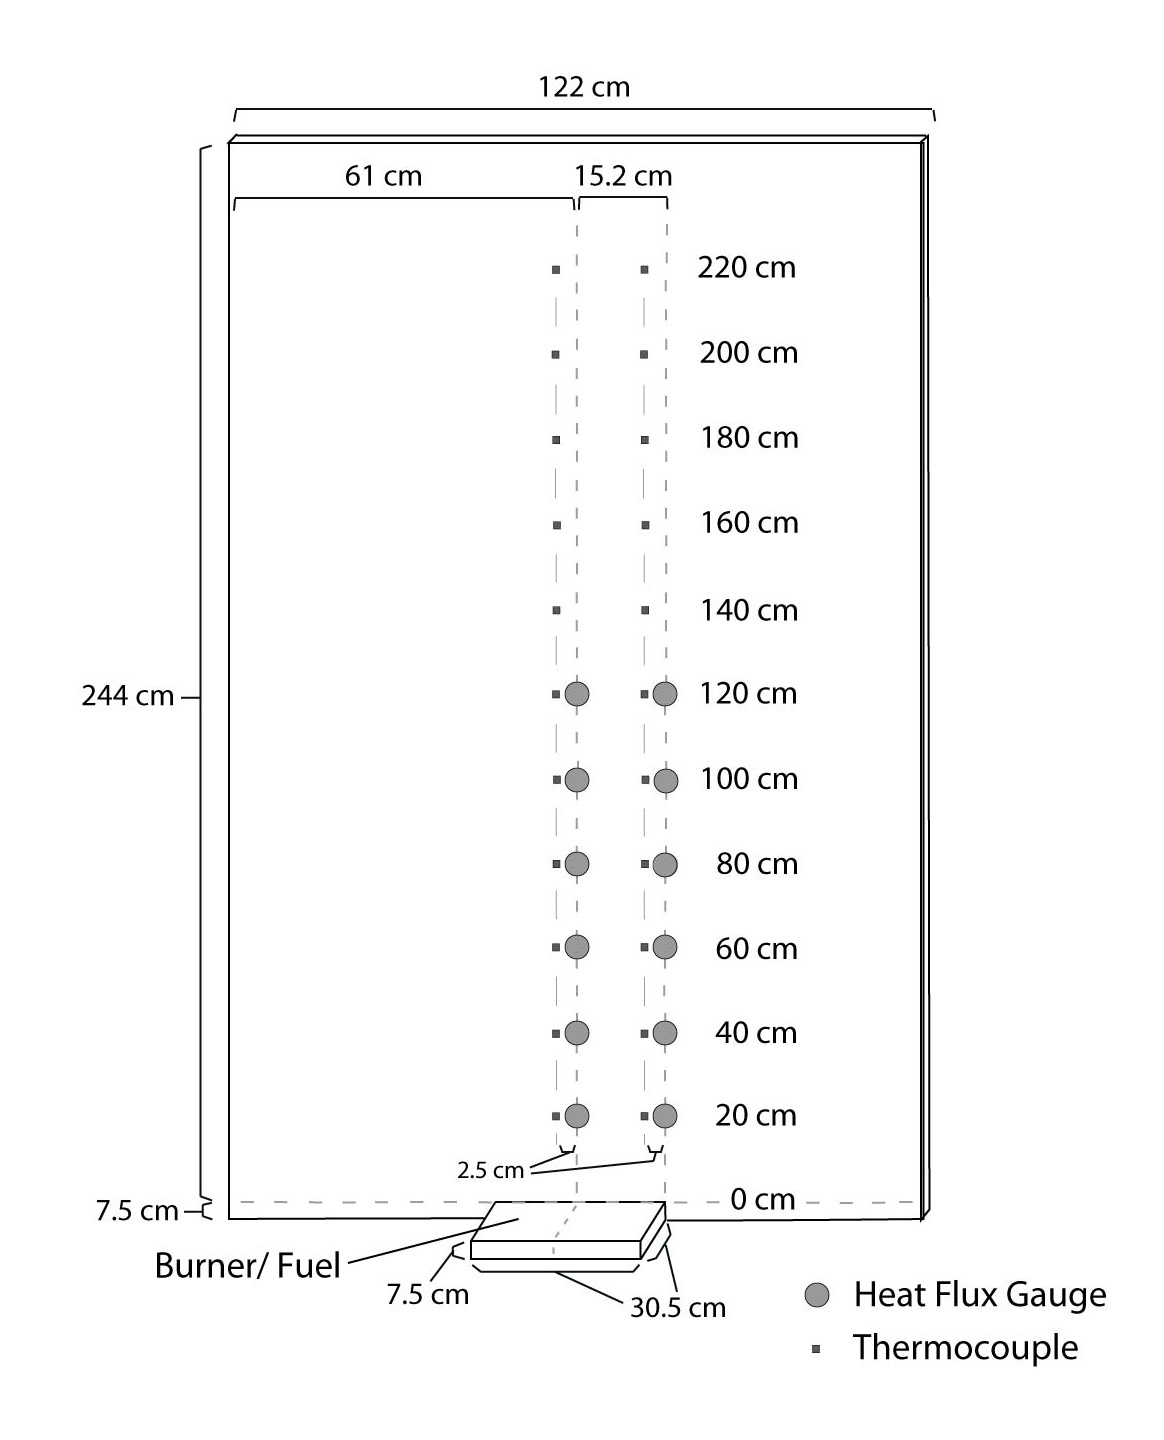
\includegraphics[width=\textwidth]{../Figures/Instrumented_NC_Wall}\\
	\caption[Diagram of the instrumented non-combustible wall]{Diagram of the instrumented non-combustible wall. Two vertical arrays of total heat flux gauges and thermocouples were installed along the centerline of the burner and along the right edge of the burner.}
	\label{Instrumented_NC_Wall}
\end{figure}

\begin{figure}
	\centering
	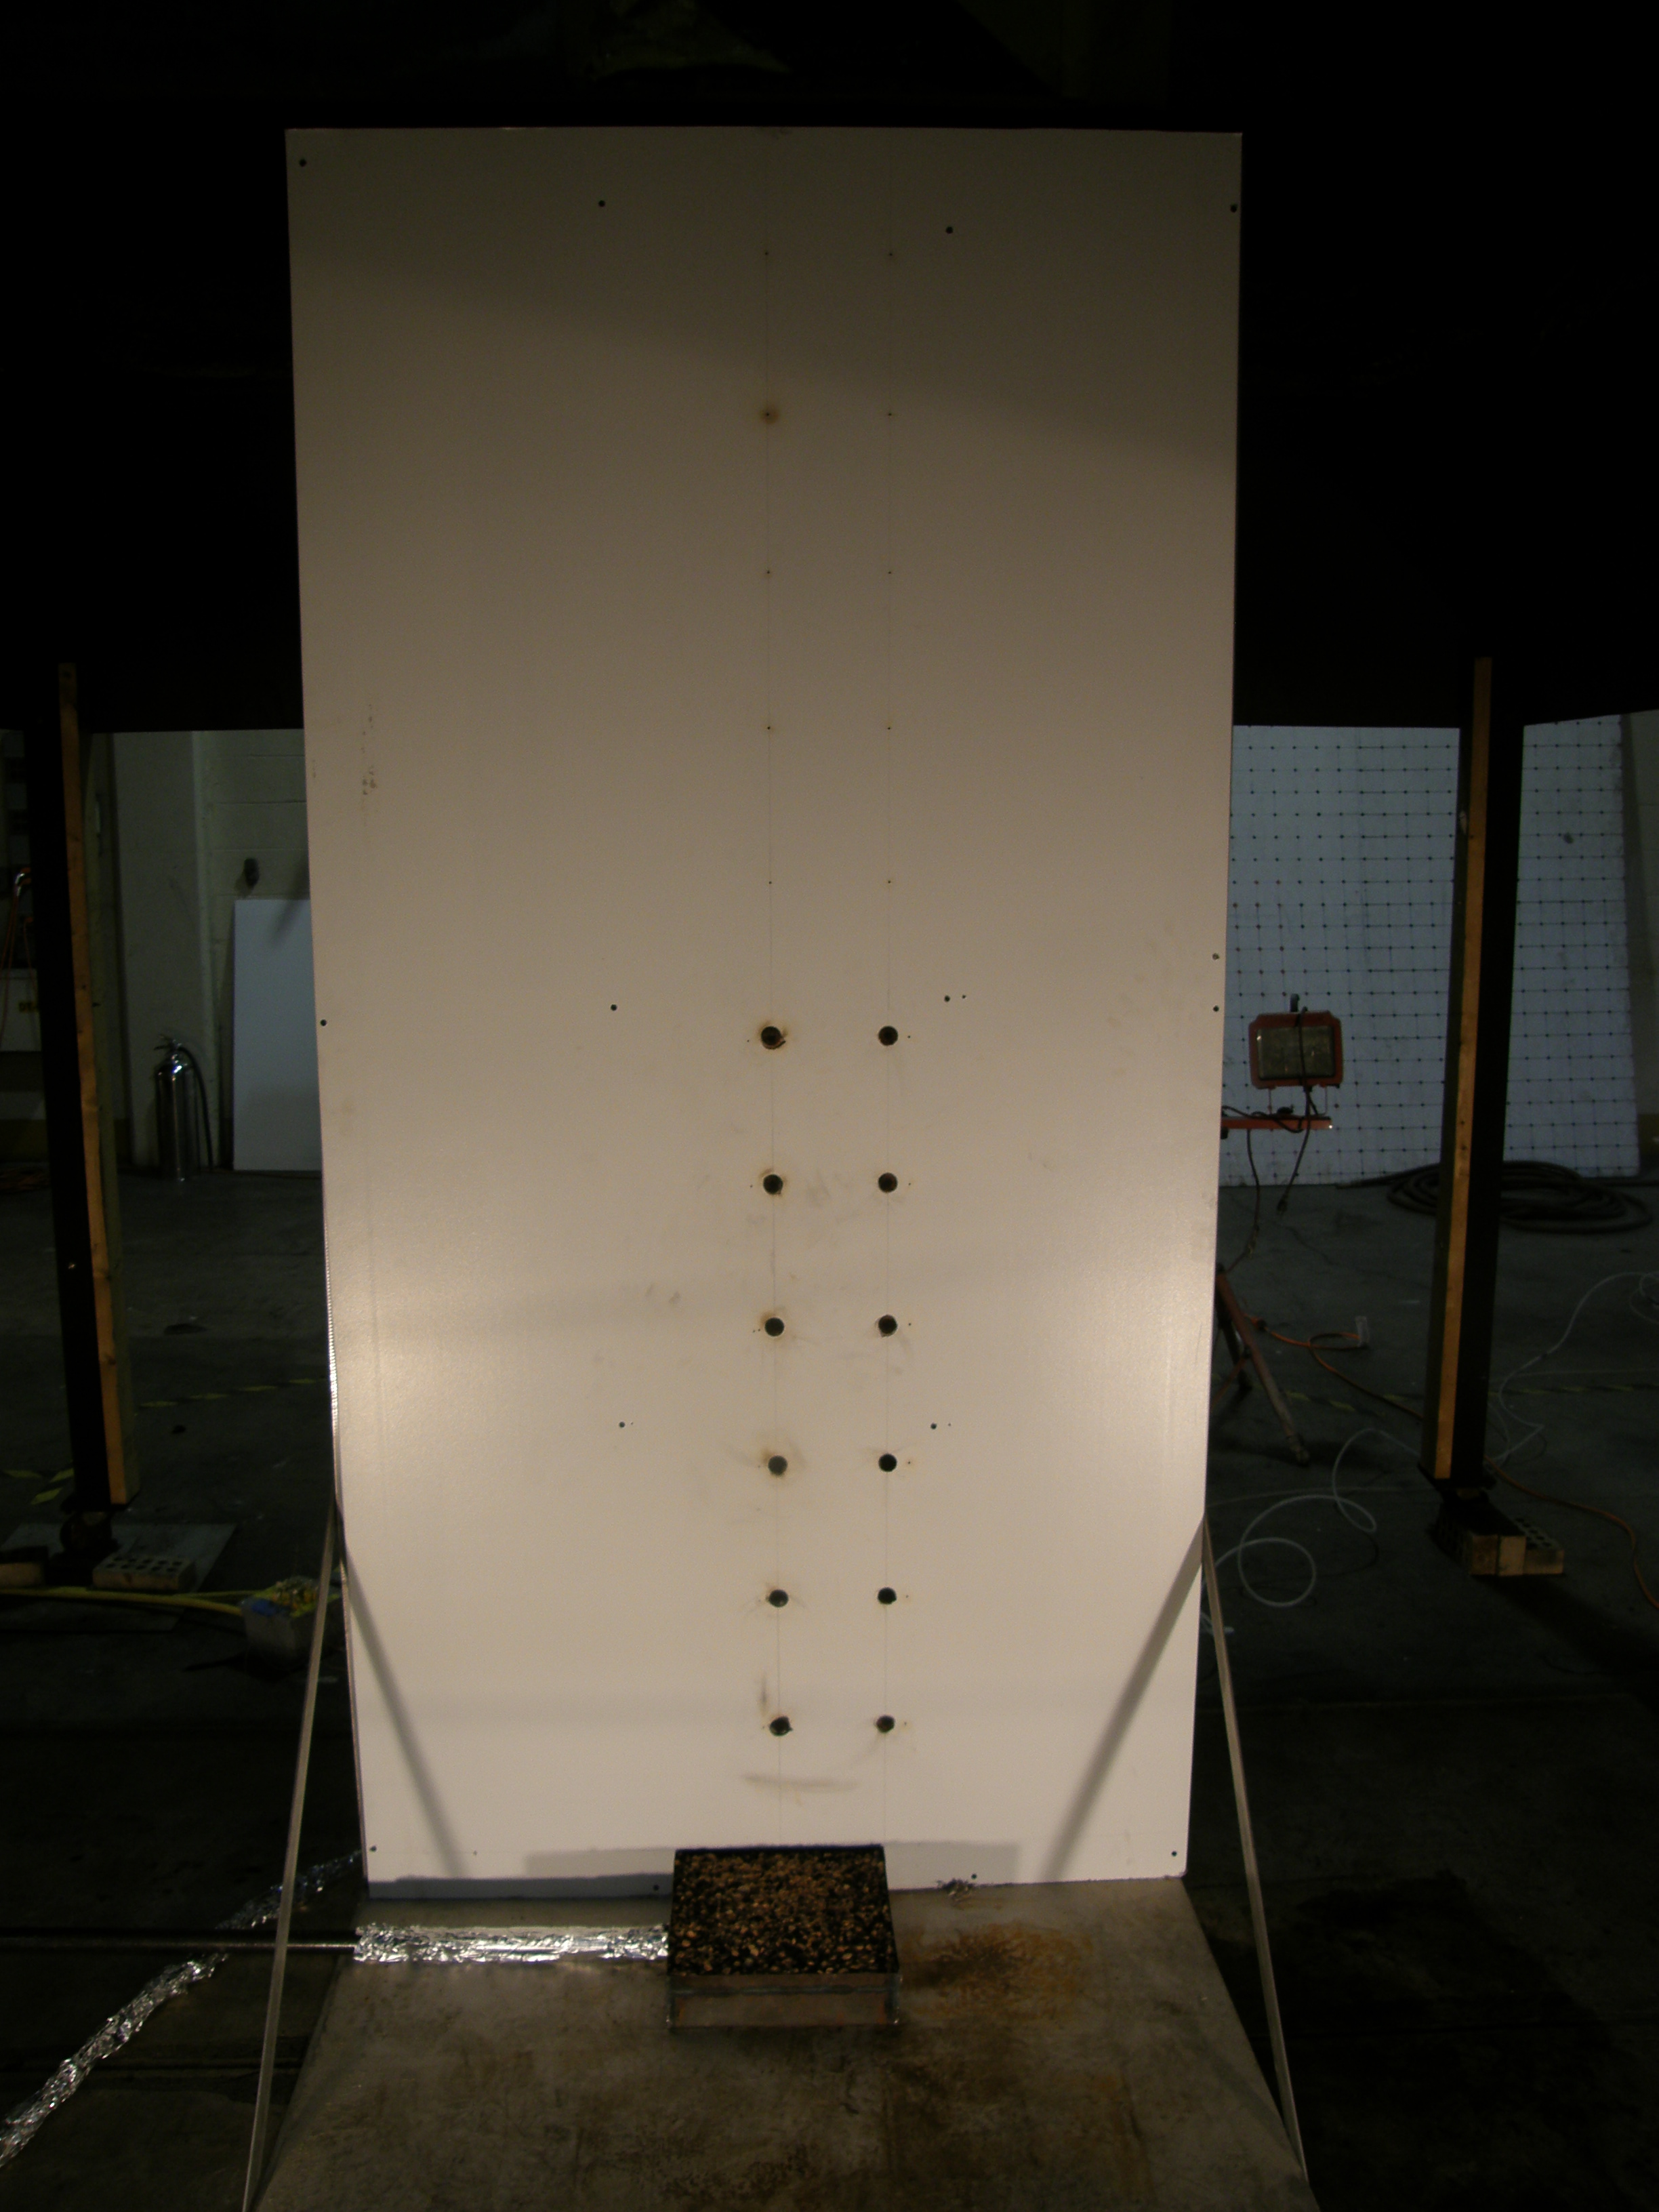
\includegraphics[width=\textwidth]{../Figures/Instrumented_Wall_Front_photo}\\
	\caption[Photograph of the front side of the instrumented non-combustible wall]{Photograph of the front side of the instrumented non-combustible wall.}
	\label{Instrumented_Wall_Front_photo}
\end{figure}


\begin{figure}
	\centering
	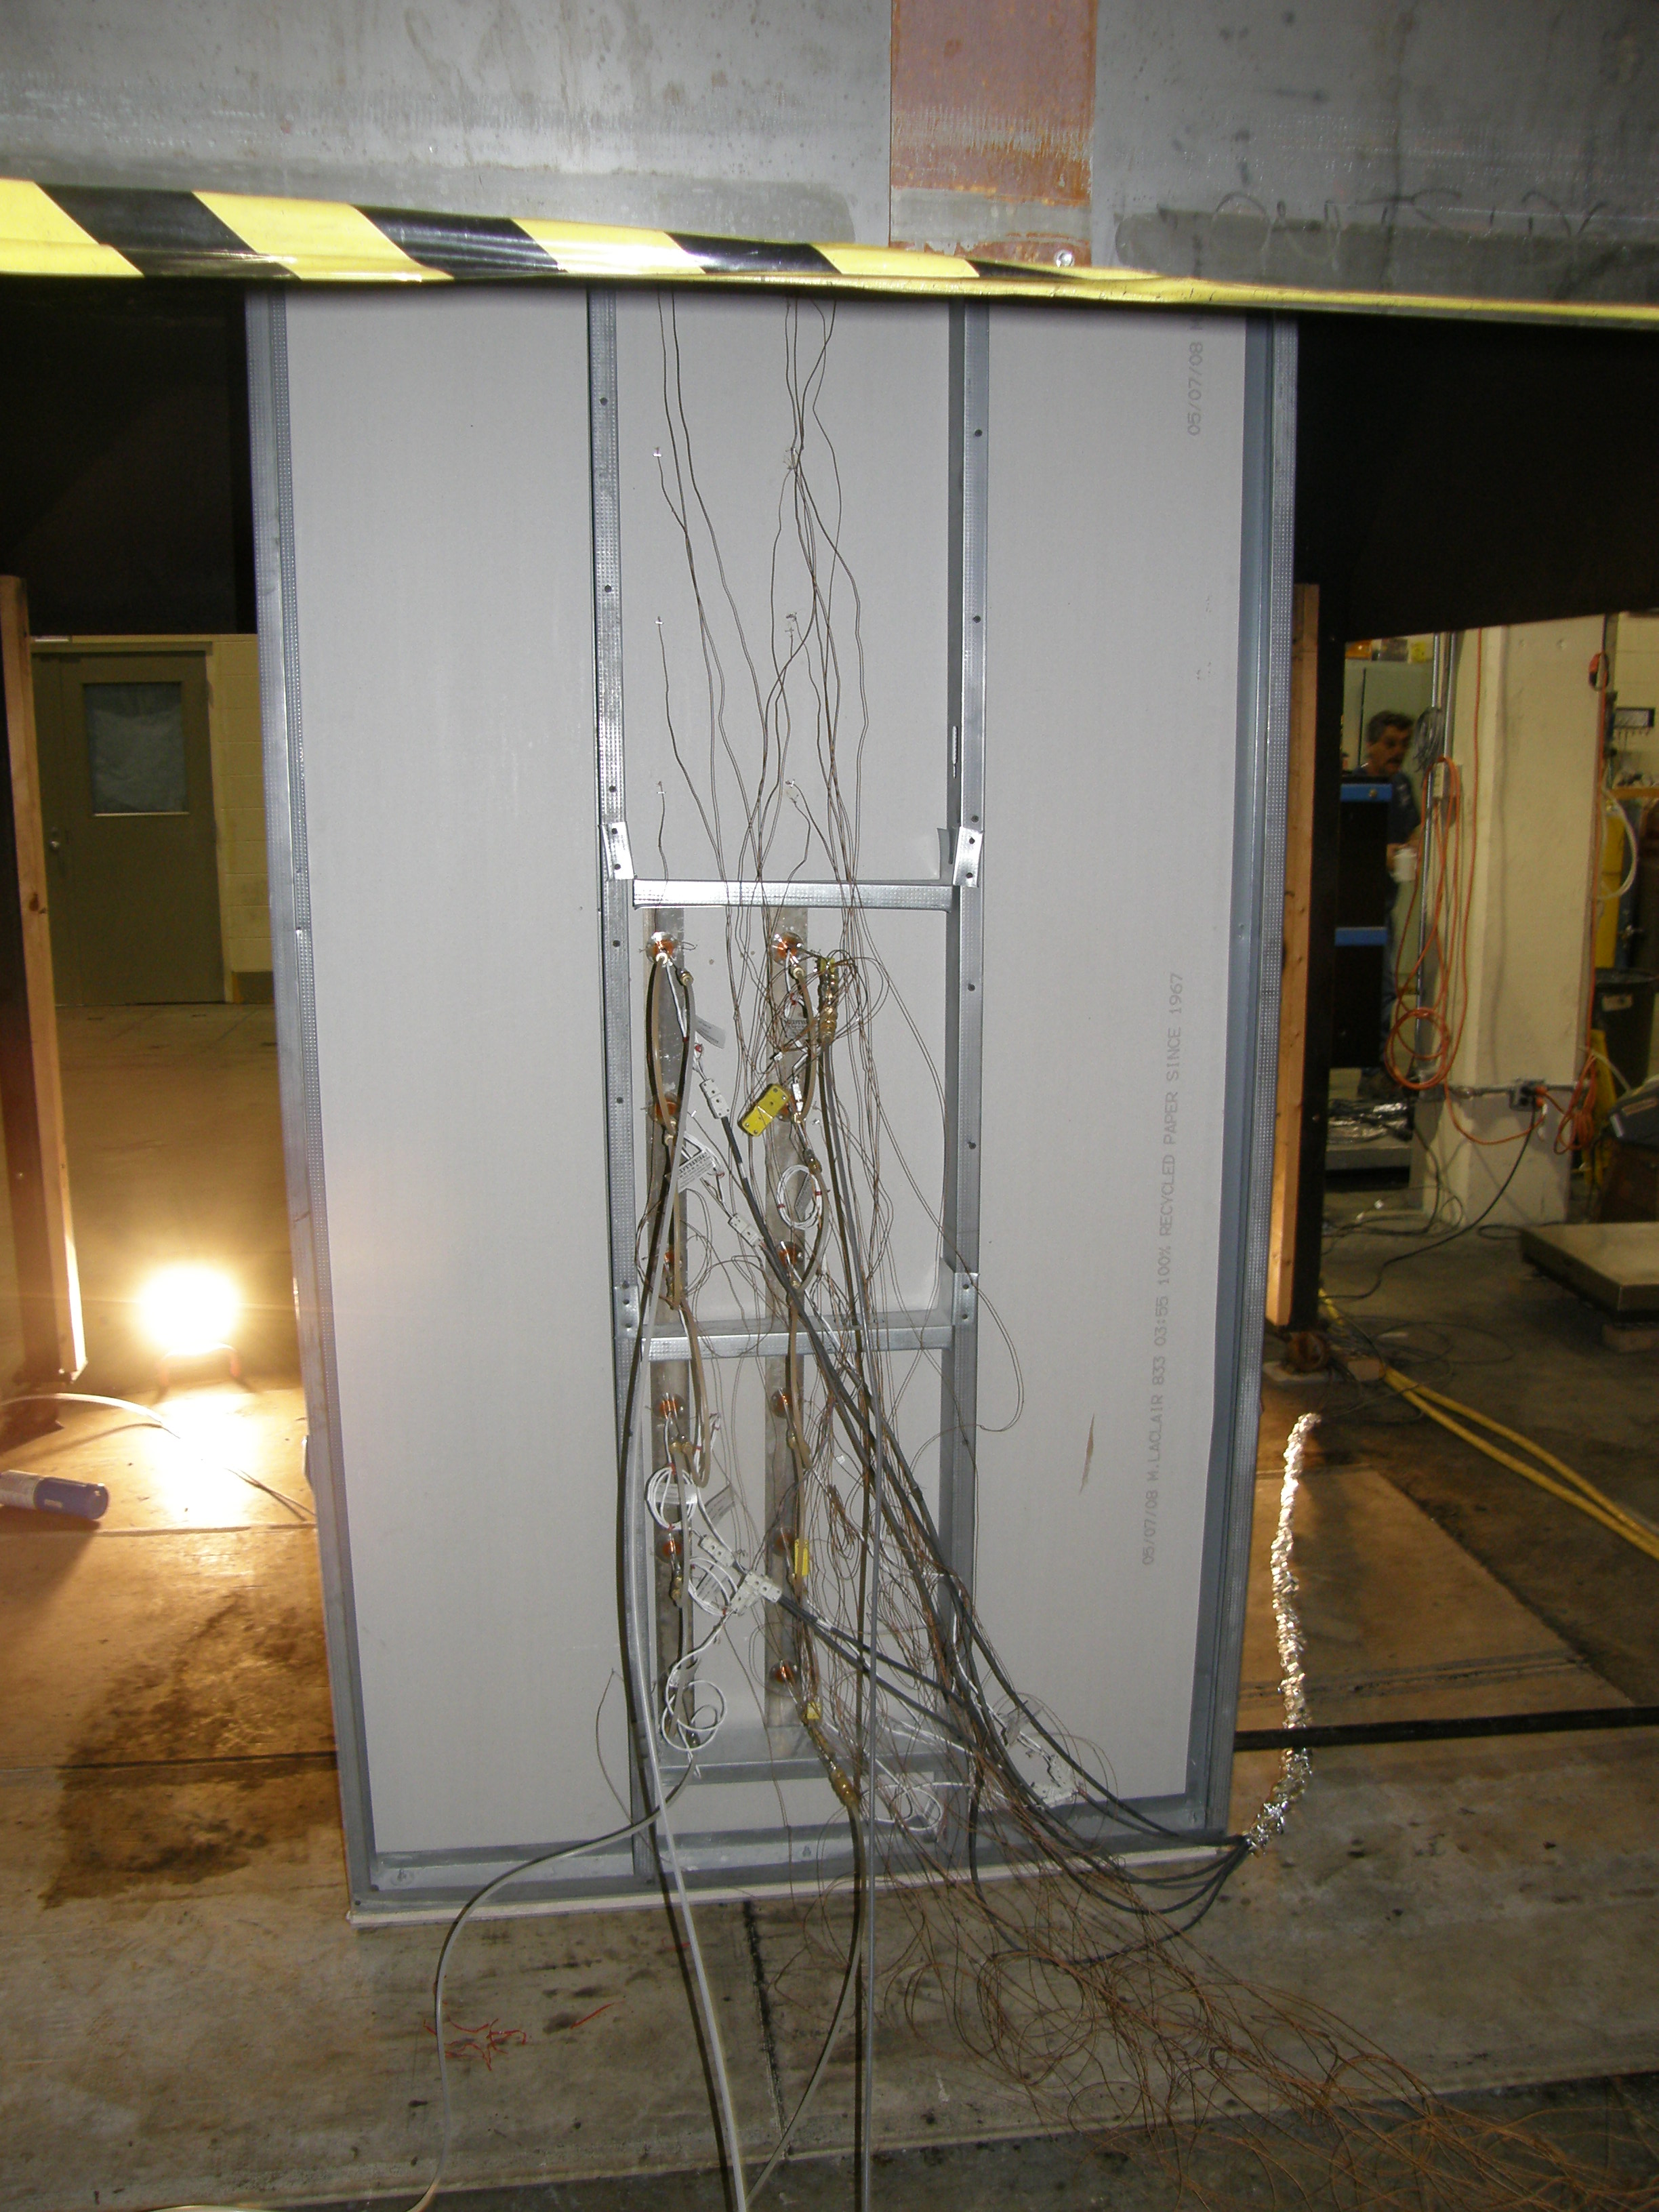
\includegraphics[width=\textwidth]{../Figures/Instrumented_Wall_Rear_photo}\\
	\caption[Photograph of the rear side of the instrumented non-combustible wall]{Photograph of the rear side of the instrumented non-combustible wall.}
	\label{Instrumented_Wall_Rear_photo}
\end{figure}



\begin{figure}
	\centering
	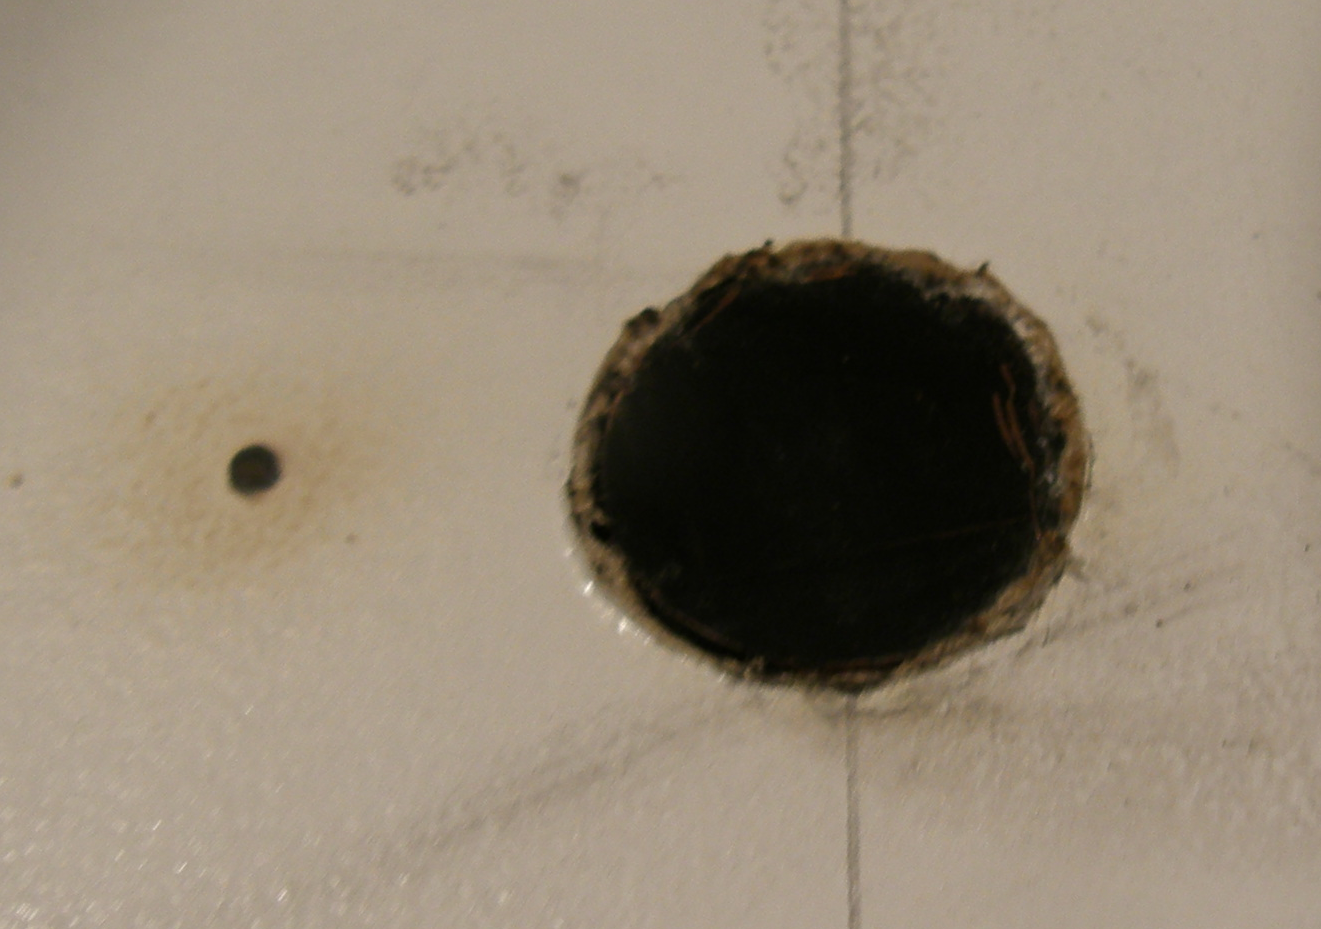
\includegraphics[width=4.0in]{../Figures/Instrumented_Wall_Close_up_TC_HF_photo}\\
	\caption[Photograph showing an example of the co-location of the heat flux gauges and the thermocouples on the front surface of the wall.]{Photograph showing an example of the co-location of the heat flux gauges and the thermocouples on the front surface of the wall.}
	\label{Instrumented_Wall_Close_up_TC_HF_photo}
\end{figure}

\begin{figure}
	\centering
	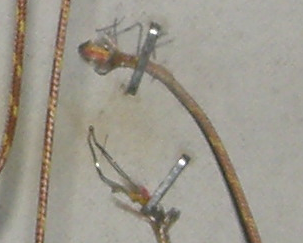
\includegraphics[width=4.0in]{../Figures/Instrumented_Wall_Detail_Rear_TC_photo}\\
	\caption[Photograph of an example of the co-location of the thermocouple on the rear surface of the wall relative to the thermocouple installed on the front surface of the wall]{Photograph of an example of the co-location of the thermocouple on the rear surface of the wall relative to the thermocouple installed on the front surface of the wall.}
	\label{Instrumented_Wall_Detail_Rear_TC_photo}
\end{figure}


\section{Results}

The results are presented for each of the four burner positions and each of the three fuels.  For the natural gas fueled experiments only two replicates were conducted at each position given the high level of control and repeatability.  For the gasoline and polyurethane fueled experiments, three replicates were conducted at each position.  The results of the wall temperatures and heat fluxes are presented as averages of the replicate experiments.  The measures of the fire including heat release rate and flame/plume temperatures were also recorded to ensure consistency with the data presented in the previous section.       

\subsection{Wall Temperatures}

\begin{figure}
	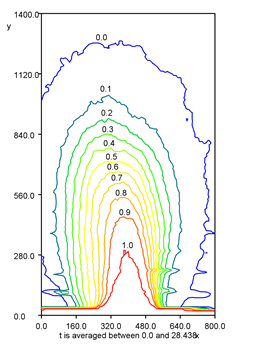
\includegraphics[width=2.7in]{../Figures/Fig20} 
	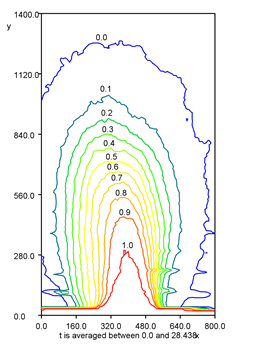
\includegraphics[width=2.7in]{../Figures/Fig21} \\
	\caption[Visibility fractions for the natural gas and gasoline fires]{Plots showing the fraction of time that the flame was visible for the natural gas (left) and gasoline (right) fires.}
	\label{Gas_and_Gasoline_Contours}
\end{figure}

\begin{figure}
	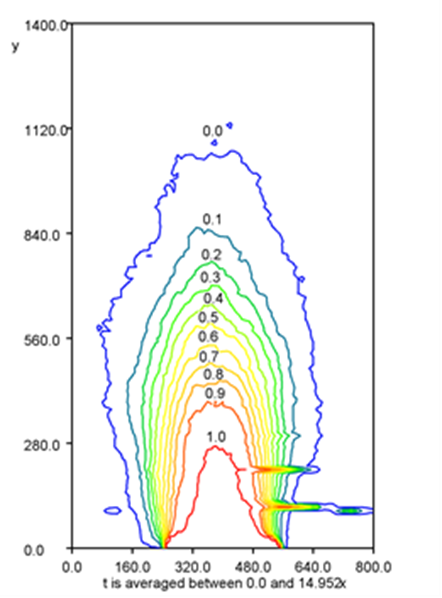
\includegraphics[width=2.7in]{../Figures/Fig22} 
	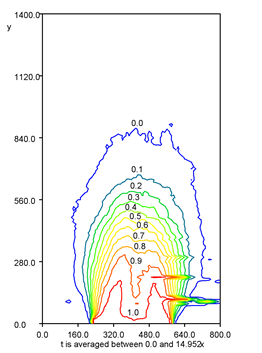
\includegraphics[width=2.7in]{../Figures/Fig23} \\
	\caption[Visibility fractions for the polyurethane foam fire]{(Left) Plot showing the fraction of time that the flame was visible for the polyurethane foam fire. (Right) Polyurethane foam contour plot with bifurcated flames at time of peak heat release rate.}
	\label{Foam_Contours}
\end{figure}


\subsection{Heat Flux}

\subsection{Fire Pattern}



\chapter{Instrumented Gypsum Board Wall Experiments}
Purpose
\section{Experimental Arrangement}
A free standing, non-combustible, steel frame with gypsum wallboard attached to the surface was instrumented to measure the thermal exposure of the wall from the fire in terms of temperature and heat flux.  The fires were initially placed at predetermined, fixed positions away from the wall. The burner was moved toward the wall until the burner was against the wall.  If the results indicated that no burn pattern would result from a given combination of fuel and position, then that fuel and position combination were eliminated from the remainder of the test matrix.

\begin{figure}
	\centering
	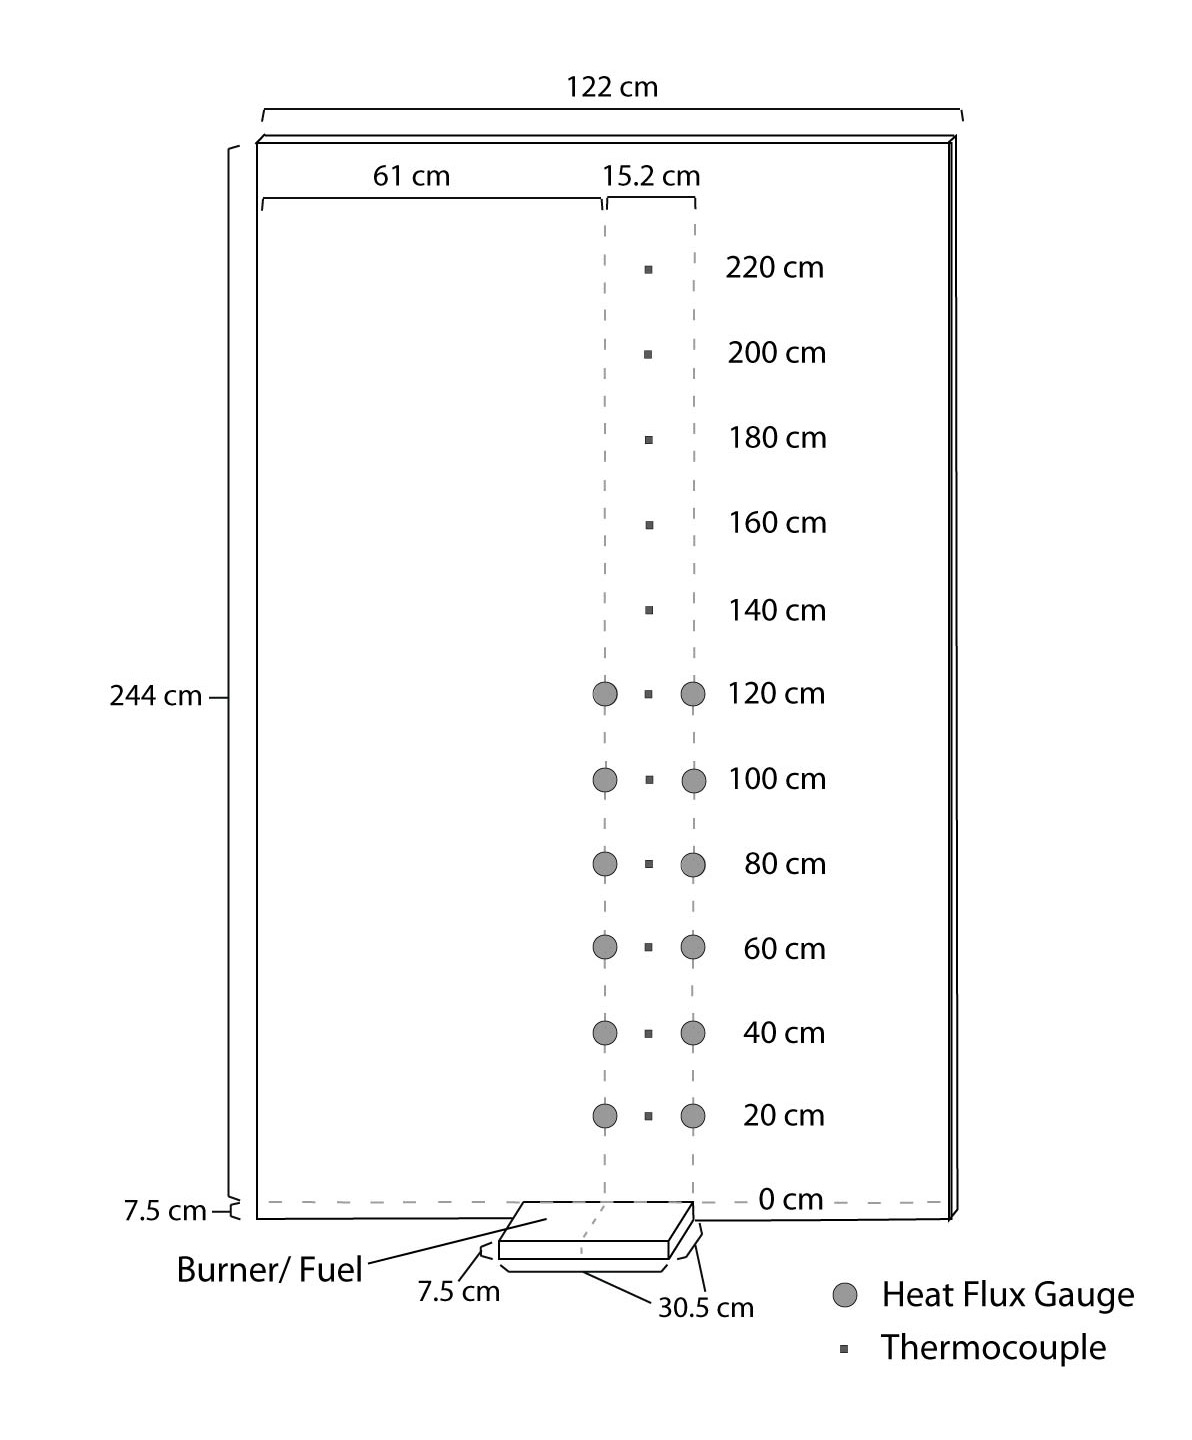
\includegraphics[width=\textwidth]{../Figures/Instrumented_GB_Wall}\\
	\caption[Diagram of the instrumented non-combustible wall]{Diagram of the instrumented non-combustible wall. Two vertical arrays of total heat flux gauges and thermocouples were installed along the centerline of the burner and along the right edge of the burner.}
	\label{Instrumented_GB_Wall}
\end{figure}






\section{Characterization of Gypsum Board}

\section{Results}

\subsection{Wall Temperatures}

\subsection{Heat Flux}

\subsection{Fire Pattern}

\chapter{Bench Scale Experiments}

\section{Cone Calorimeter Experiments}

\section{Radiant Flooring Panel Experiments}

\section{Radiant Panel Experiments}

\section{Results}

\subsection{Ignition Temperature}

\subsection{Heat Release Rate per Unit Area}

\subsection{Critical Heat Flux}


\chapter{Fire Pattern Compartment Experiments}

\section{Wall Construction Type Experiments}
\subsection{Experimental Arrangement}
\subsection{Results}

\section{Wall Position Experiments}
\subsection{Experimental Arrangement}

\subsection{Results}

\subsubsection{Natural Gas}
\subsubsection{Gasoline}
\subsubsection{Polyurethane Foam}

\section{Corner Position Experiments}

\subsection{Experimental Arrangement}

\subsection{Results}

\subsubsection{Natural Gas}
\subsubsection{Gasoline}
\subsubsection{Polyurethane Foam}

\chapter{Summary of Experimental Results}

Needed?

\chapter{Comparison of Algebraic Fire Characterizations with Fire Pattern Results}

\section{Evidence of a Fire Pattern}

\section{Flame Height Correlation}

\subsection{Correlation Descriptions}

\section{Comparison of Results}

\chapter{Comparison of Field Model Simulations with Experimental Results}

\section{Fire Dynamics Simulator and Smokeview}

\subsection{Simulation of Fires}

\subsection{Input Data}

\section{Comparison of FDS with Source Fire Results}

\subsection{Grid Size Analysis}

\subsection{Plume Temperatures}

\subsection{Heat Flux}

\subsection{Flame Height}

\section{Comparison of FDS with Fire Pattern Results} 

\chapter{Discussion}

\chapter{Future Research Needs}

\chapter{Conclusions}





\bibliography{../References/Madrzykowski_Thesis}
\end{document}
